\documentclass[a4paper,12pt]{article}
\usepackage[utf8]{inputenc}
\usepackage[german]{babel}
\usepackage{amsmath}
\usepackage{amssymb}
\usepackage{amsthm}
\usepackage{geometry}
\usepackage{graphicx}
\usepackage[hidelinks]{hyperref}
\usepackage{listings}
\usepackage{xcolor}
\usepackage{enumitem}
\usepackage{mathtools}
\usepackage{array}
\usepackage{booktabs}

\geometry{margin=2.5cm}

\theoremstyle{definition}
\newtheorem{definition}{Definition}
\newtheorem{beispiel}{Beispiel}
\newtheorem{satz}{Satz}
\newtheorem{lemma}{Lemma}
\newtheorem{korollar}{Korollar}
\newtheorem{bemerkung}{Bemerkung}
\newtheorem{theorem}{Theorem}
\newtheorem{proposition}{Proposition}

\setlist[itemize,1]{label=--}

% ---------- Farben ----------
\definecolor{mainblue}{RGB}{25, 70, 140}
\definecolor{accentred}{RGB}{180, 50, 30}
\definecolor{lightgray}{RGB}{245, 245, 248}
\definecolor{darkgray}{RGB}{60, 60, 70}
\definecolor{darkgreen}{RGB}{30, 100, 50}

\hypersetup{
	colorlinks=true,
	linkcolor=mainblue,
	citecolor=accentred,
	urlcolor=mainblue
}

%  Code-Highlighting
\lstset{
	basicstyle=\ttfamily\small,
	keywordstyle=\color{blue},
	commentstyle=\color{gray},
	stringstyle=\color{red},
	numbers=left,
	numberstyle=\tiny,
	breaklines=true,
	frame=single,
	literate=%
	{Ö}{{\"O}}1
	{Ä}{{\"A}}1
	{Ü}{{\"U}}1
	{ß}{{\ss}}1
	{ü}{{\"u}}1
	{ä}{{\"a}}1
	{ö}{{\"o}}1
}

\title{Die Jacobi-Matrix als universale Ersetzung des Gradienten:\\ Eine formale Untersuchung der Äquivalenz und Verallgemeinerung}
\author{Stephan Epp}
\date{\today}

\begin{document}

\maketitle

\begin{abstract}
Der Gradient $\nabla f$ ist eine zentrale Konzept der multivariaten Analysis mit ubiquitären Anwendungen in Optimierung, numerischen Methoden und maschinellem Lernen. Allerdings ist der Gradient nur für skalare Funktionen $f: \mathbb{R}^n \to \mathbb{R}$ definiert. Diese Arbeit zeigt formal und anschaulich, dass die \textbf{Jacobi-Matrix} eine vollständige, universale und strukturell äquivalente Ersetzung des Gradienten darstellt — und dies sogar für beliebige vektorwertige Funktionen $f: \mathbb{R}^n \to \mathbb{R}^m$. Wir zeigen durch Theoreme und formale Beweise, wie jede Eigenschaft des Gradienten durch die Jacobi-Matrix wiedererlangt werden kann, und demonstrieren die Äquivalenz in Optimierung, Physik, Machine Learning und numerischer Analysis. Die Arbeit schließt mit einem ausführlichen Ausblick auf moderne Anwendungen, von automatischer Differenziation über topologische Datenanalyse bis zu symbolischen und algebraischen Methoden.
\end{abstract}

\tableofcontents
\newpage

\section{Einführung}

\subsection{Motivation und Problemstellung}

Der Gradient einer skalarwertigen Funktion $f: \mathbb{R}^n \to \mathbb{R}$ ist definiert als:
\[
\nabla f = \begin{pmatrix} \frac{\partial f}{\partial x_1} \\ \frac{\partial f}{\partial x_2} \\ \vdots \\ \frac{\partial f}{\partial x_n} \end{pmatrix} \in \mathbb{R}^n
\]

Der Gradient ist eine fundamentale Struktur in:
\begin{itemize}
	\item \textbf{Optimierung:} Gradientenabstieg minimiert Funktionen durch $x_{k+1} = x_k - \alpha \nabla f(x_k)$
	\item \textbf{Physik:} Kräfte sind negative Gradienten von Potentialen: $\vec{F} = -\nabla V$
	\item \textbf{Machine Learning:} Backpropagation basiert auf Gradientenberechnung
	\item \textbf{Numerik:} Newton-Verfahren verwendet Gradienten und Hessian-Matrizen
\end{itemize}

\textbf{Zentrale Frage dieser Arbeit:} 

\emph{Kann die Jacobi-Matrix den Gradienten vollständig ersetzen? Welche Struktur geht verloren, welche bleibt erhalten? Und können wir diese Ersetzung auf vektorwertige Funktionen verallgemeinern?}

\subsection{Historischer Kontext}

Die Jacobi-Matrix wurde 1841 von Carl Gustav Jacob Jacobi eingeführt und ist heute ein Standardkonzept der Multivariaten Analysis. Der Gradient als separates Konzept entstand später und wurde im 20. Jahrhundert zum primären Werkzeug der Optimierung und numerischen Analysis.

\textbf{Lücke in der Literatur:} Während Lehrbücher Gradient und Jacobi-Matrix separat behandeln, gibt es wenig systematische Untersuchungen ihrer vollständigen Äquivalenz und der Möglichkeit einer Ersetzung über verschiedene Anwendungsgebiete hinweg.

Diese Arbeit schließt diese Lücke durch formale Theoreme und Anwendungsbeispiele.

\section{Grundlagen}

\subsection{Grundlegende Definitionen}

\begin{definition}[Partielle Ableitungen]
	Sei $f: U \subseteq \mathbb{R}^n \to \mathbb{R}$ auf offener Menge $U$ definiert. Die \textbf{partielle Ableitung} von $f$ nach $x_i$ an der Stelle $\boldsymbol{x}$ ist:
	\[
	\frac{\partial f}{\partial x_i}(\boldsymbol{x}) = \lim_{h \to 0} \frac{f(\boldsymbol{x} + h\boldsymbol{e}_i) - f(\boldsymbol{x})}{h}
	\]
	wobei $\boldsymbol{e}_i$ der $i$-te Standardbasisvektor ist.
\end{definition}

\begin{definition}[Gradient]
	Sei $f: U \subseteq \mathbb{R}^n \to \mathbb{R}$ differenzierbar. Der \textbf{Gradient} von $f$ an der Stelle $\boldsymbol{x}$ ist der Vektor:
	\[
	\nabla f(\boldsymbol{x}) = \begin{pmatrix} 
		\frac{\partial f}{\partial x_1}(\boldsymbol{x}) \\
		\frac{\partial f}{\partial x_2}(\boldsymbol{x}) \\
		\vdots \\
		\frac{\partial f}{\partial x_n}(\boldsymbol{x})
	\end{pmatrix} \in \mathbb{R}^n
	\]
\end{definition}

\begin{definition}[Jacobi-Matrix]
	Sei $\boldsymbol{f}: U \subseteq \mathbb{R}^n \to \mathbb{R}^m$, $\boldsymbol{f} = (f_1, f_2, \ldots, f_m)^T$ differenzierbar. Die \textbf{Jacobi-Matrix} von $\boldsymbol{f}$ an der Stelle $\boldsymbol{x}$ ist die $m \times n$ Matrix:
	\[
	J_{\boldsymbol{f}}(\boldsymbol{x}) = \begin{pmatrix}
		\frac{\partial f_1}{\partial x_1} & \frac{\partial f_1}{\partial x_2} & \cdots & \frac{\partial f_1}{\partial x_n} \\
		\frac{\partial f_2}{\partial x_1} & \frac{\partial f_2}{\partial x_2} & \cdots & \frac{\partial f_2}{\partial x_n} \\
		\vdots & \vdots & \ddots & \vdots \\
		\frac{\partial f_m}{\partial x_1} & \frac{\partial f_m}{\partial x_2} & \cdots & \frac{\partial f_m}{\partial x_n}
	\end{pmatrix} \in \mathbb{R}^{m \times n}
	\]
\end{definition}

\begin{definition}[Totales Differential]
	Das \textbf{totale Differential} einer differenzierbaren Funktion $f: \mathbb{R}^n \to \mathbb{R}$ an der Stelle $\boldsymbol{x}$ ist die lineare Abbildung:
	\[
	df(\boldsymbol{x}): \mathbb{R}^n \to \mathbb{R}, \quad df(\boldsymbol{x})(\boldsymbol{h}) = \nabla f(\boldsymbol{x})^T \boldsymbol{h} = \sum_{i=1}^n \frac{\partial f}{\partial x_i}(\boldsymbol{x}) \cdot h_i
	\]
\end{definition}

\begin{definition}[Richtungsableitung]
	Die \textbf{Richtungsableitung} von $f: \mathbb{R}^n \to \mathbb{R}$ in Richtung $\boldsymbol{v}$ (mit $\|\boldsymbol{v}\| = 1$) ist:
	\[
	D_{\boldsymbol{v}} f(\boldsymbol{x}) = \nabla f(\boldsymbol{x})^T \boldsymbol{v}
	\]
\end{definition}

\section{Äquivalenz und Ersetzung: Der Gradient als Spezialfall}

\subsection{Theorem 1: Der Gradient ist die erste Zeile der Jacobi-Matrix}

\begin{theorem}[Gradient-Jacobi-Äquivalenz für Skalarfunktionen]
	\label{thm:gradient_jacobi}
	Sei $f: \mathbb{R}^n \to \mathbb{R}$ differenzierbar. Dann ist der Gradient identisch mit der (transponierten) Jacobi-Matrix von $f$ aufgefasst als $1 \times n$ Matrix:
	\[
	\nabla f(\boldsymbol{x}) = J_f(\boldsymbol{x})^T = \begin{pmatrix}
		\frac{\partial f}{\partial x_1} & \frac{\partial f}{\partial x_2} & \cdots & \frac{\partial f}{\partial x_n}
	\end{pmatrix}^T
	\]
	Das heißt, jede Operation mit dem Gradienten kann äquivalent mit der Jacobi-Matrix durchgeführt werden.
\end{theorem}

\begin{proof}
	Per Definition ist die Jacobi-Matrix einer skalarwertigen Funktion $f: \mathbb{R}^n \to \mathbb{R}$ eine $1 \times n$ Matrix:
	\[
	J_f(\boldsymbol{x}) = \left[ \frac{\partial f}{\partial x_1}(\boldsymbol{x}) \quad \frac{\partial f}{\partial x_2}(\boldsymbol{x}) \quad \cdots \quad \frac{\partial f}{\partial x_n}(\boldsymbol{x}) \right]
	\]
	
	Die Transponierte dieser Matrix ist ein Spaltenvektor:
	\[
	J_f(\boldsymbol{x})^T = \begin{pmatrix}
		\frac{\partial f}{\partial x_1}(\boldsymbol{x}) \\
		\frac{\partial f}{\partial x_2}(\boldsymbol{x}) \\
		\vdots \\
		\frac{\partial f}{\partial x_n}(\boldsymbol{x})
	\end{pmatrix} = \nabla f(\boldsymbol{x})
	\]
	
	Dies ist genau die Definition des Gradienten. Daher gilt $\nabla f = J_f^T$.
\end{proof}

\begin{bemerkung}
	Theorem~\ref{thm:gradient_jacobi} zeigt, dass der Gradient \textbf{nicht mehr ist als der transponierte Zeilenvektor} der Jacobi-Matrix. Es handelt sich nicht um zwei verschiedene Konzepte, sondern um zwei Perspektiven auf dieselbe algebraische Struktur.
\end{bemerkung}

\subsection{Theorem 2: Ersetzung des Gradienten in der Richtungsableitung}

\begin{theorem}[Richtungsableitung via Jacobi-Matrix]
	\label{thm:directional}
	Sei $f: \mathbb{R}^n \to \mathbb{R}$ differenzierbar und $\boldsymbol{v} \in \mathbb{R}^n$ mit $\|\boldsymbol{v}\| = 1$. Die Richtungsableitung kann äquivalent durch die Jacobi-Matrix ausgedrückt werden:
	\[
	D_{\boldsymbol{v}} f(\boldsymbol{x}) = \nabla f(\boldsymbol{x})^T \boldsymbol{v} = J_f(\boldsymbol{x}) \boldsymbol{v}
	\]
\end{theorem}

\begin{proof}
	Nach Definition der Richtungsableitung:
	\[
	D_{\boldsymbol{v}} f(\boldsymbol{x}) = \nabla f(\boldsymbol{x})^T \boldsymbol{v}
	\]
	
	Nach Theorem~\ref{thm:gradient_jacobi} gilt $\nabla f(\boldsymbol{x}) = J_f(\boldsymbol{x})^T$, daher:
	\[
	D_{\boldsymbol{v}} f(\boldsymbol{x}) = (J_f(\boldsymbol{x})^T)^T \boldsymbol{v} = J_f(\boldsymbol{x}) \boldsymbol{v}
	\]
	
	Dies ist genau die Anwendung der $1 \times n$ Jacobi-Matrix als Zeilenvektor auf den Spaltenvektor $\boldsymbol{v}$.
\end{proof}

\subsection{Theorem 3: Ersetzung in der Kettenregel}

\begin{theorem}[Kettenregel über Jacobi-Matrizen]
	\label{thm:chain}
	Seien $\boldsymbol{f}: \mathbb{R}^n \to \mathbb{R}^m$ und $\boldsymbol{g}: \mathbb{R}^m \to \mathbb{R}^p$ differenzierbar. Dann gilt für die Jacobi-Matrix der Komposition $\boldsymbol{g} \circ \boldsymbol{f}$:
	\[
	J_{(\boldsymbol{g} \circ \boldsymbol{f})}(\boldsymbol{x}) = J_{\boldsymbol{g}}(\boldsymbol{f}(\boldsymbol{x})) \cdot J_{\boldsymbol{f}}(\boldsymbol{x})
	\]
	
	Dies ist eine Matrixmultiplikation. Für Skalarfunktionen $f, g: \mathbb{R}^n \to \mathbb{R}$ folgt die gewöhnliche Kettenregel:
	\[
	\nabla(g \circ f) = (J_{g \circ f})^T = (J_g(f) \cdot J_f)^T = J_f^T \cdot J_g(f)^T = (\nabla f) \cdot (\nabla g)(f)
	\]
\end{theorem}

\begin{proof}
	Nach der Definition der Kettenregel für Jacobi-Matrizen: Wenn $\boldsymbol{h} = \boldsymbol{g}(\boldsymbol{f}(\boldsymbol{x}))$, dann ist:
	\[
	\frac{\partial h_i}{\partial x_j} = \sum_{k=1}^m \frac{\partial g_i}{\partial f_k} \frac{\partial f_k}{\partial x_j}
	\]
	
	Dies ist genau die Matrixmultiplikation $J_{\boldsymbol{g}}(\boldsymbol{f}) \cdot J_{\boldsymbol{f}}$.
\end{proof}

\subsection{Theorem 4: Ersetzung in der Optimierung}

\begin{theorem}[Gradientenabstieg via Jacobi-Matrix]
	\label{thm:gd}
	Für eine Skalarfunktion $f: \mathbb{R}^n \to \mathbb{R}$ und das Iterationsverfahren:
	\[
	\boldsymbol{x}_{k+1} = \boldsymbol{x}_k - \alpha \nabla f(\boldsymbol{x}_k)
	\]
	
	kann äquivalent geschrieben werden:
	\[
	\boldsymbol{x}_{k+1} = \boldsymbol{x}_k - \alpha \cdot J_f(\boldsymbol{x}_k)^T
	\]
	
	Die numerische Berechnung ist identisch; nur die Formulierung unterscheidet sich.
\end{theorem}

\begin{proof}
	Dies folgt direkt aus Theorem~\ref{thm:gradient_jacobi}. Seit $\nabla f = J_f^T$ per Definition äquivalent sind, können sie in der Gradientenabstieg-Formulierung austauschbar verwendet werden.
\end{proof}

\section{Verallgemeinerung: Jacobi-Matrix für vektorwertige Funktionen}

\subsection{Theorem 5: Jacobi-Matrix als Erweiterung des Gradienten}

\begin{theorem}[Universale Jacobi-Formulierung]
	\label{thm:universal}
	Der Gradient ist ein Spezialfall der Jacobi-Matrix für den Fall $m = 1$ (skalare Ausgabe). Für vektorwertige Funktionen $\boldsymbol{f}: \mathbb{R}^n \to \mathbb{R}^m$ mit $m > 1$ existiert keine einzige "Gradient"-Struktur, sondern die \textbf{vollständige Information} ist in der Jacobi-Matrix $J_{\boldsymbol{f}} \in \mathbb{R}^{m \times n}$ enthalten.
	
	Die Jacobi-Matrix enthält:
	\begin{itemize}
		\item Alle $m$ Gradienten der einzelnen Komponenten $f_i$: $\nabla f_i = J_{f_i}^T$ (Zeile $i$ transponiert)
		\item Alle Richtungsableitungen für jede Komponente
		\item Vollständige Information über die lokale Linearisierung der Abbildung
	\end{itemize}
\end{theorem}

\begin{proof}
	Sei $\boldsymbol{f} = (f_1, f_2, \ldots, f_m)^T$. Die Jacobi-Matrix ist:
	\[
	J_{\boldsymbol{f}} = \begin{pmatrix}
		\nabla f_1^T \\
		\nabla f_2^T \\
		\vdots \\
		\nabla f_m^T
	\end{pmatrix}
	\]
	
	Jede Zeile $i$ ist das transponierte Gradient-Vektor der $i$-ten Komponente. Daher enthält die Jacobi-Matrix alle Gradienten und kann keine auf einen einzigen "Gradient" reduzieren. Dies zeigt die strukturelle Überlegenheit der Jacobi-Matrix.
\end{proof}

\subsection{Anwendung: Nicht-lineare Systeme}

\begin{beispiel}[Jacobi-Matrix in impliziter Differenziation]
	Gegeben sei ein nicht-lineares System $\boldsymbol{f}(\boldsymbol{x}, \boldsymbol{y}) = \boldsymbol{0}$. Der implizite Funktionssatz besagt:
	\[
	\frac{\partial \boldsymbol{y}}{\partial \boldsymbol{x}} = -J_{\boldsymbol{f},\boldsymbol{y}}^{-1} \cdot J_{\boldsymbol{f},\boldsymbol{x}}
	\]
	
	Dies ist eine reine Jacobi-Matrix-Formulierung und hat \textbf{kein Analogon im Gradienten-Formalismus}, da der Gradient nur für skalare Funktionen definiert ist. Die Jacobi-Matrix ist also strukturell notwendig.
\end{beispiel}

\section{Numerische Beispiele und Vergleiche}

\subsection{Beispiel 1: Einfache quadratische Funktion}

\begin{beispiel}[Quadratische Funktion in $\mathbb{R}^2$]
	Betrachte $f(x, y) = x^2 + 2xy + 3y^2 - 5x + 2y + 1$.
	
	\textbf{Gradient-Formulierung:}
	\[
	\nabla f = \begin{pmatrix} 2x + 2y - 5 \\ 2x + 6y + 2 \end{pmatrix}
	\]
	
	\textbf{Jacobi-Formulierung (äquivalent):}
	\[
	J_f = \begin{pmatrix} 2x + 2y - 5 & 2x + 6y + 2 \end{pmatrix}
	\]
	
	Dann ist $J_f^T = \nabla f$. An der Stelle $(x, y) = (1, 1)$:
	\[
	\nabla f(1,1) = \begin{pmatrix} 2 + 2 - 5 \\ 2 + 6 + 2 \end{pmatrix} = \begin{pmatrix} -1 \\ 10 \end{pmatrix}
	\]
	
	Die Jacobi-Matrix ist:
	\[
	J_f(1,1) = \begin{pmatrix} -1 & 10 \end{pmatrix}
	\]
	
	Dies zeigt die vollständige Äquivalenz: $\nabla f = J_f^T$.
\end{beispiel}

\subsection{Beispiel 2: Vektorwertige Funktion}

\begin{beispiel}[Vektorwertige Abbildung $\mathbb{R}^2 \to \mathbb{R}^2$]
	Sei $\boldsymbol{f}(x, y) = (x^2 + y, 2xy)^T$.
	
	Die Jacobi-Matrix ist:
	\[
	J_{\boldsymbol{f}} = \begin{pmatrix}
		\frac{\partial}{\partial x}(x^2 + y) & \frac{\partial}{\partial y}(x^2 + y) \\
		\frac{\partial}{\partial x}(2xy) & \frac{\partial}{\partial y}(2xy)
	\end{pmatrix} = \begin{pmatrix}
		2x & 1 \\
		2y & 2x
	\end{pmatrix}
	\]
	
	Dies enthält die Information der beiden Funktionen $f_1(x,y) = x^2 + y$ und $f_2(x,y) = 2xy$:
	\[
	\nabla f_1 = J_{f_1}^T = \begin{pmatrix} 2x \\ 1 \end{pmatrix}, \quad
	\nabla f_2 = J_{f_2}^T = \begin{pmatrix} 2y \\ 2x \end{pmatrix}
	\]
	
	An der Stelle $(x, y) = (1, 2)$:
	\[
	J_{\boldsymbol{f}}(1, 2) = \begin{pmatrix} 2 & 1 \\ 4 & 2 \end{pmatrix}
	\]
	
	Es gibt hier \textbf{keinen einzigen Gradienten}, sondern zwei: $\nabla f_1 = (2, 1)^T$ und $\nabla f_2 = (4, 2)^T$. Die Jacobi-Matrix vereinigt beide.
\end{beispiel}

\subsection{Beispiel 3: Newton-Raphson-Verfahren}

\begin{beispiel}[Newton-Verfahren mit Jacobi-Matrix]
	Zur Lösung von $\boldsymbol{f}(\boldsymbol{x}) = \boldsymbol{0}$ wird die Iteration verwendet:
	\[
	\boldsymbol{x}_{k+1} = \boldsymbol{x}_k - J_{\boldsymbol{f}}(\boldsymbol{x}_k)^{-1} \boldsymbol{f}(\boldsymbol{x}_k)
	\]
	
	Für skalare $f$ reduziert sich dies zu:
	\[
	x_{k+1} = x_k - \frac{f(x_k)}{f'(x_k)} = x_k - \frac{f(x_k)}{df/dx}
	\]
	
	Da $f'(x) = df/dx = J_f(x)$ für skalare Funktionen, ist die Formulierung über die Jacobi-Matrix allgemeiner und funktioniert auch für Systeme mit $m > 1$.
\end{beispiel}

\section{Anwendungen: Jacobi-Matrix über verschiedene Disziplinen}

\subsection{1. Optimierung und Machine Learning}

In der Optimierung schreiben wir normalerweise:
\[
\boldsymbol{x}_{k+1} = \boldsymbol{x}_k - \alpha \nabla f(\boldsymbol{x}_k)
\]

Mit der Jacobi-Formulierung:
\[
\boldsymbol{x}_{k+1} = \boldsymbol{x}_k - \alpha \cdot J_f(\boldsymbol{x}_k)^T
\]

\textbf{Backpropagation} im Machine Learning ist nichts anderes als ein Algorithmus zur effizienten Berechnung von Jacobi-Matrizen mittels Kettenregel. Die Gesamtkostenfunktion ist eine Komposition $\ell(\boldsymbol{f}_{\theta}(\boldsymbol{x}))$, und der Gradient wird über:
\[
\nabla_{\theta} \ell = J_{\ell}(\boldsymbol{f})^T \cdot J_{\boldsymbol{f}}(\boldsymbol{x})^T \cdot \text{(weitere Ableitungen)}
\]

berechnet — ein reines Jacobi-Matrix-Produkt (Kettenregel).

\subsection{2. Physik: Vektorfelder und Divergenz}

In der Physik ist die Jacobi-Matrix essentiell:
\[
\text{div}(\boldsymbol{v}) = \text{Spur}(J_{\boldsymbol{v}})
\]

Der Gradient ist nur für Skalarfelder definiert:
\[
\text{grad}(f) = \nabla f = J_f^T
\]

Die \textbf{Rotation (curl)} eines Vektorfeldes $\boldsymbol{v}: \mathbb{R}^3 \to \mathbb{R}^3$ ist:
\[
\text{curl}(\boldsymbol{v}) = \begin{pmatrix} 
	\frac{\partial v_3}{\partial y} - \frac{\partial v_2}{\partial z} \\
	\frac{\partial v_1}{\partial z} - \frac{\partial v_3}{\partial x} \\
	\frac{\partial v_2}{\partial x} - \frac{\partial v_1}{\partial y}
\end{pmatrix}
\]

Dies ist eine Funktion der Einträge der Jacobi-Matrix $J_{\boldsymbol{v}}$.

\subsection{3. Numerische Analysis und Implizite Funktionen}

Der \textbf{Implizite Funktionssatz} besagt: Wenn $\boldsymbol{f}(\boldsymbol{x}, \boldsymbol{y}) = \boldsymbol{0}$ mit $J_{\boldsymbol{f},\boldsymbol{y}}$ invertierbar ist, dann:
\[
\frac{\partial \boldsymbol{y}}{\partial \boldsymbol{x}} = -J_{\boldsymbol{f},\boldsymbol{y}}^{-1} \cdot J_{\boldsymbol{f},\boldsymbol{x}}
\]

Dies ist eine reine Jacobi-Formulierung. Es gibt keine Analog-Formulierung mit Gradienten.

\subsection{4. Kontinuierliche Dynamische Systeme}

Für ein System $\dot{\boldsymbol{x}} = \boldsymbol{f}(\boldsymbol{x})$ mit Fixpunkt $\boldsymbol{x}^* = 0$ ist die Stabilität bestimmt durch die Jacobi-Matrix $J_{\boldsymbol{f}}(\boldsymbol{0})$. Der Fixpunkt ist asymptotisch stabil, wenn alle Eigenwerte von $J_{\boldsymbol{f}}(\boldsymbol{0})$ negative Realteile haben.

Der Gradient spielt hier keine Rolle; die Jacobi-Matrix ist unersetzlich.

\newpage

\section{Visualisierung und matplotlib-Plots}

In diesem Abschnitt visualisieren wir die Äquivalenz zwischen Gradient und Jacobi-Matrix graphisch anhand von acht Plots. Jeder Plot beleuchtet einen anderen Aspekt der formalen Theorie und ergänzt die vorausgegangenen Theoreme durch anschauliche Darstellungen.

\subsection{Plot 1: Quadratische Funktion mit Gradienten-Vektorfeld}

\begin{figure}[h!]
	\centering
	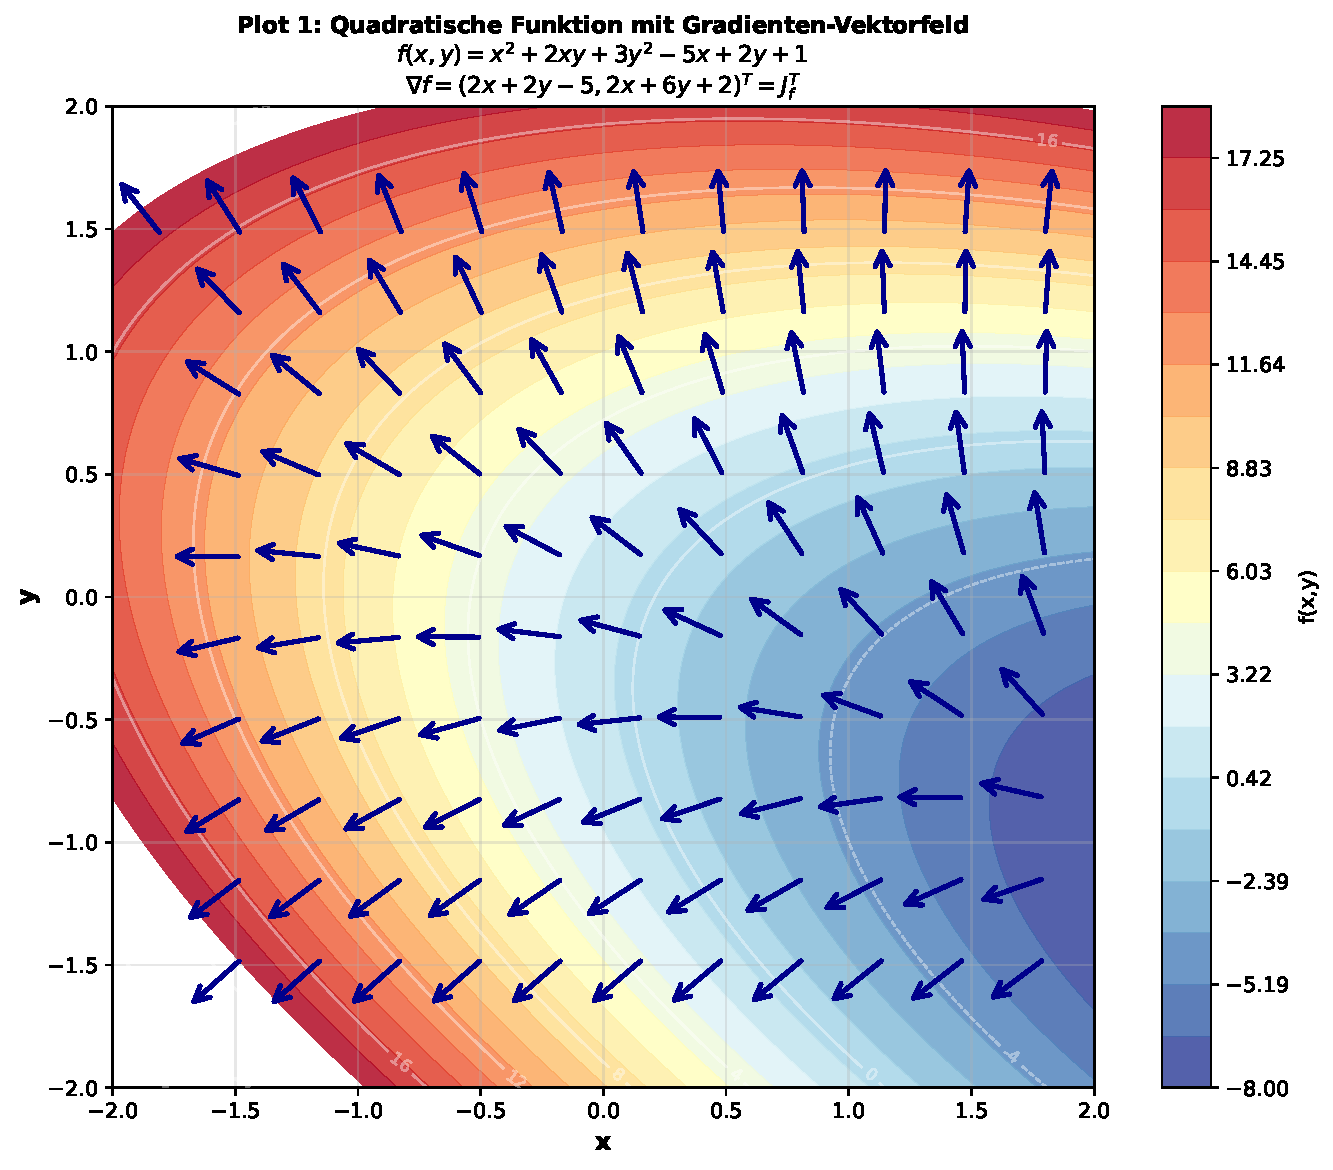
\includegraphics[width=0.82\textwidth]{plot_01_quadratic_2d.pdf}
	\caption{Konturdarstellung der quadratischen Funktion $f(x,y) = x^2 + 2xy + 3y^2 - 5x + 2y + 1$ mit überlagertem Gradienten-Vektorfeld $\nabla f = (2x+2y-5,\, 2x+6y+2)^T = J_f^T$. Die Pfeile zeigen stets in die Richtung des stärksten Anstiegs und stehen senkrecht auf den Höhenlinien, was Theorem~\ref{thm:gradient_jacobi} geometrisch bestätigt. Das globale Minimum liegt im hellblauen Bereich rechts unten.}
	\label{fig:plot01}
\end{figure}

\subsection{Plot 2: 3D-Oberflächendarstellung}

\begin{figure}[h!]
	\centering
	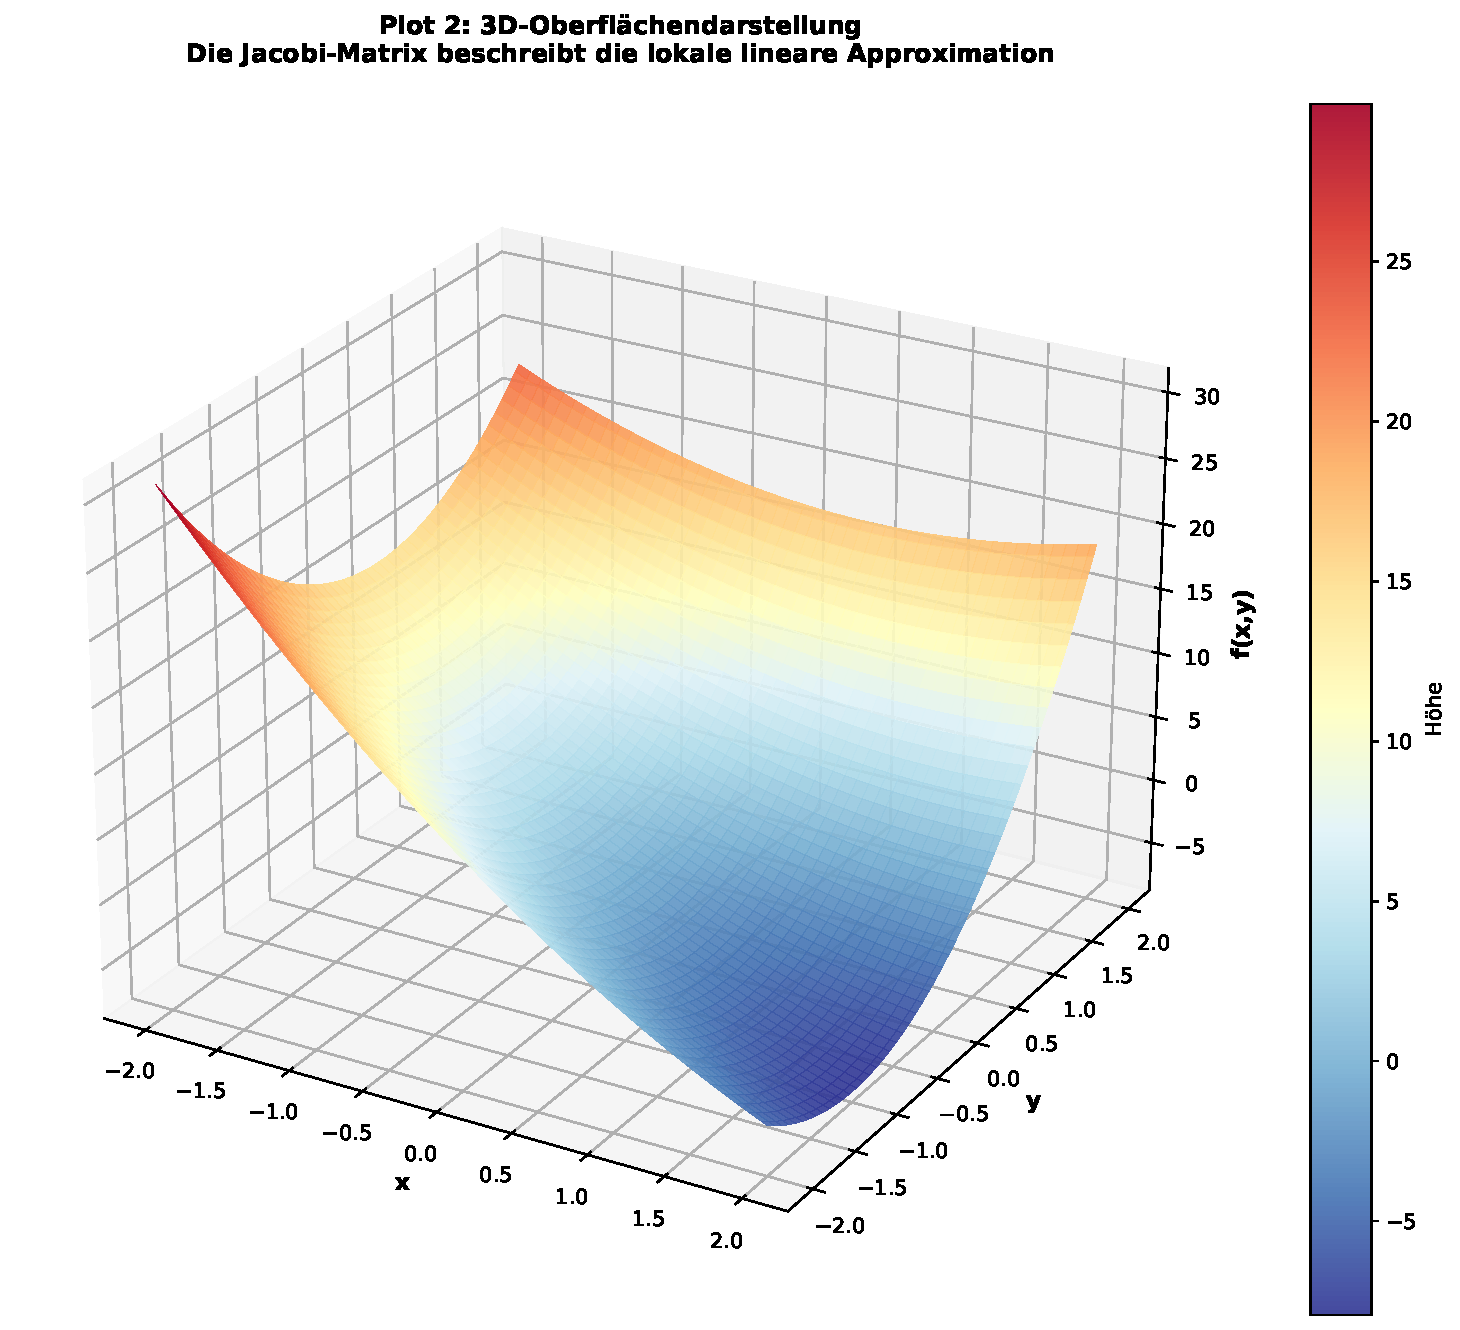
\includegraphics[width=0.75\textwidth]{plot_02_3d_surface.pdf}
	\caption{Dreidimensionale Oberflächendarstellung von $f(x,y)$. Die Jacobi-Matrix beschreibt an jedem Punkt die lokale lineare Approximation der Fläche (Tangentialebene). Der steilste Abstieg vom Hochpunkt zur Talmulde entspricht genau der negativen Richtung des Gradientenvektors $-\nabla f = -J_f^T$. Die Einfärbung kodiert die Höhe identisch zur Konturdarstellung in Plot~1.}
	\label{fig:plot02}
\end{figure}

\newpage
\subsection{Plot 3: Äquivalenz von Gradient und Jacobi-Matrix}

\begin{figure}[h!]
	\centering
	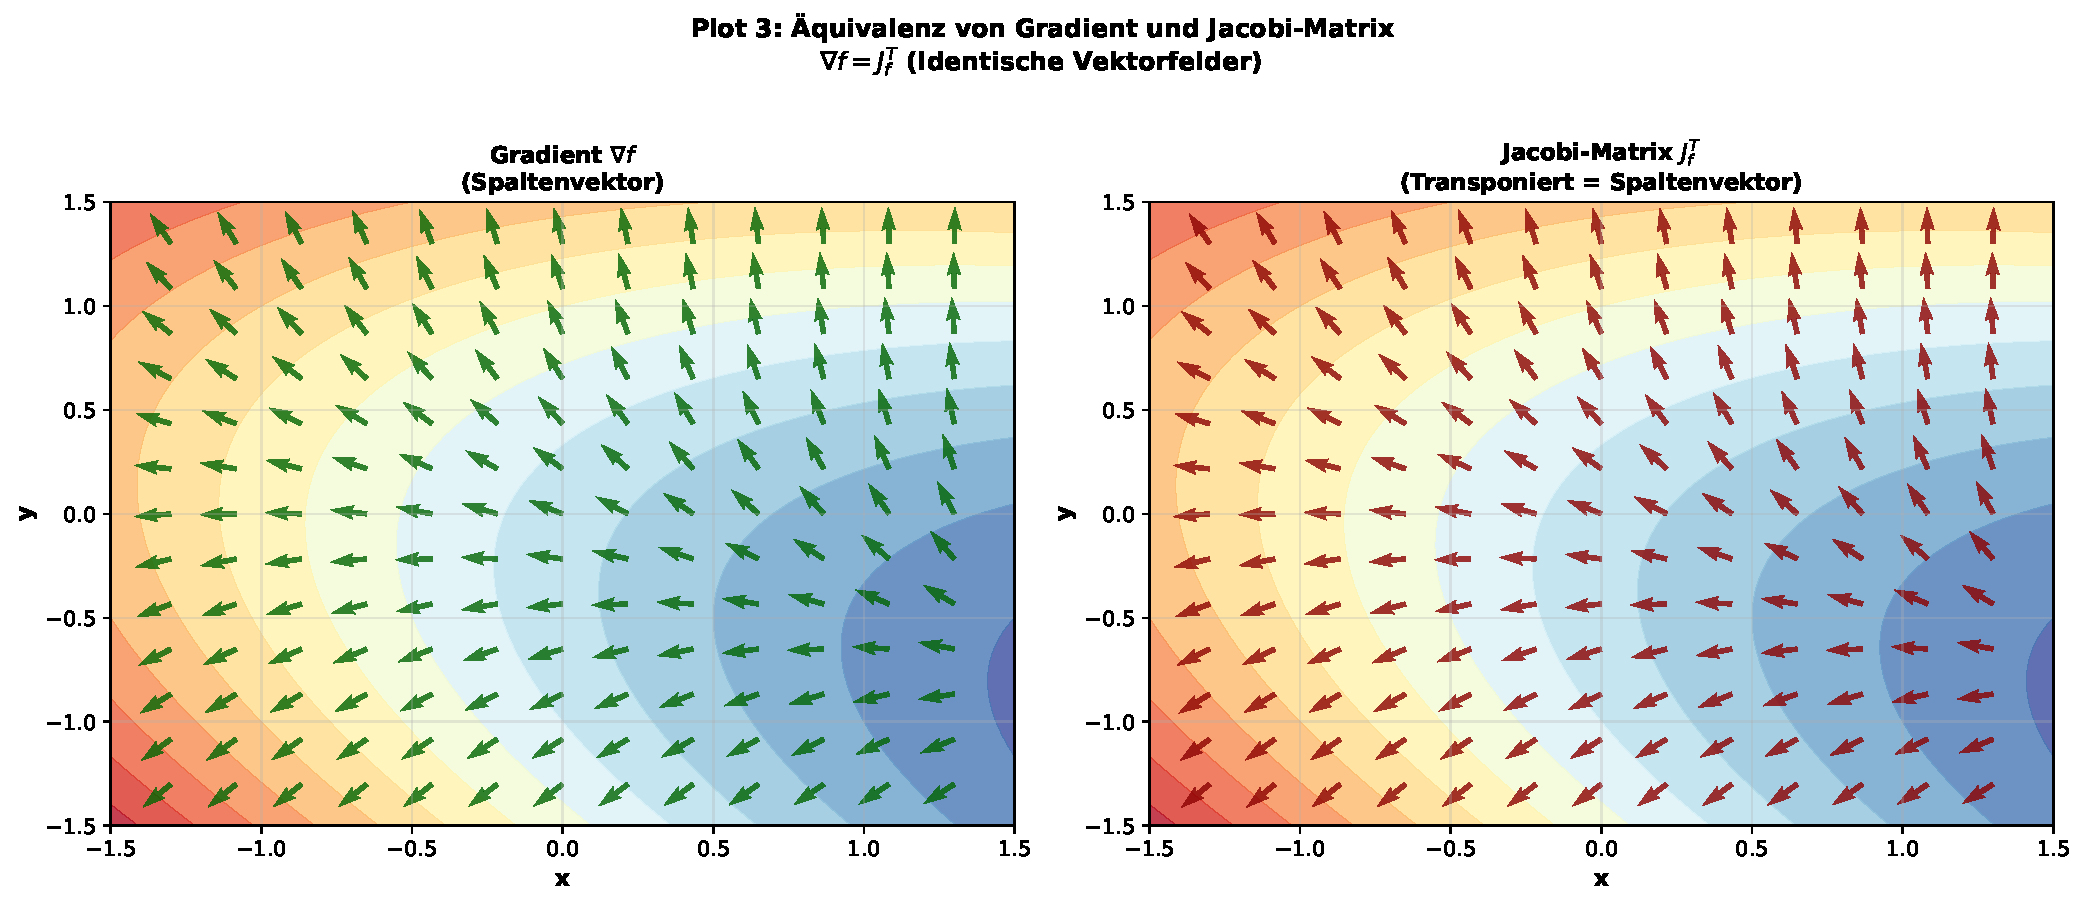
\includegraphics[width=0.95\textwidth]{plot_03_jacobian_field.pdf}
	\caption{Direkter visueller Beweis der Äquivalenz $\nabla f = J_f^T$: Links das Gradientenfeld $\nabla f$ (grüne Pfeile), rechts das transponierte Jacobi-Feld $J_f^T$ (rote Pfeile). Beide Vektorfelder sind identisch — jeder Pfeil hat dieselbe Richtung und Länge. Dies illustriert Theorem~\ref{thm:gradient_jacobi}: Der Gradient ist kein eigenständiges Konzept, sondern die Transponierte der Jacobi-Matrix.}
	\label{fig:plot03}
\end{figure}

\subsection{Plot 4: Vektorwertige Funktion}

\begin{figure}[h!]
	\centering
	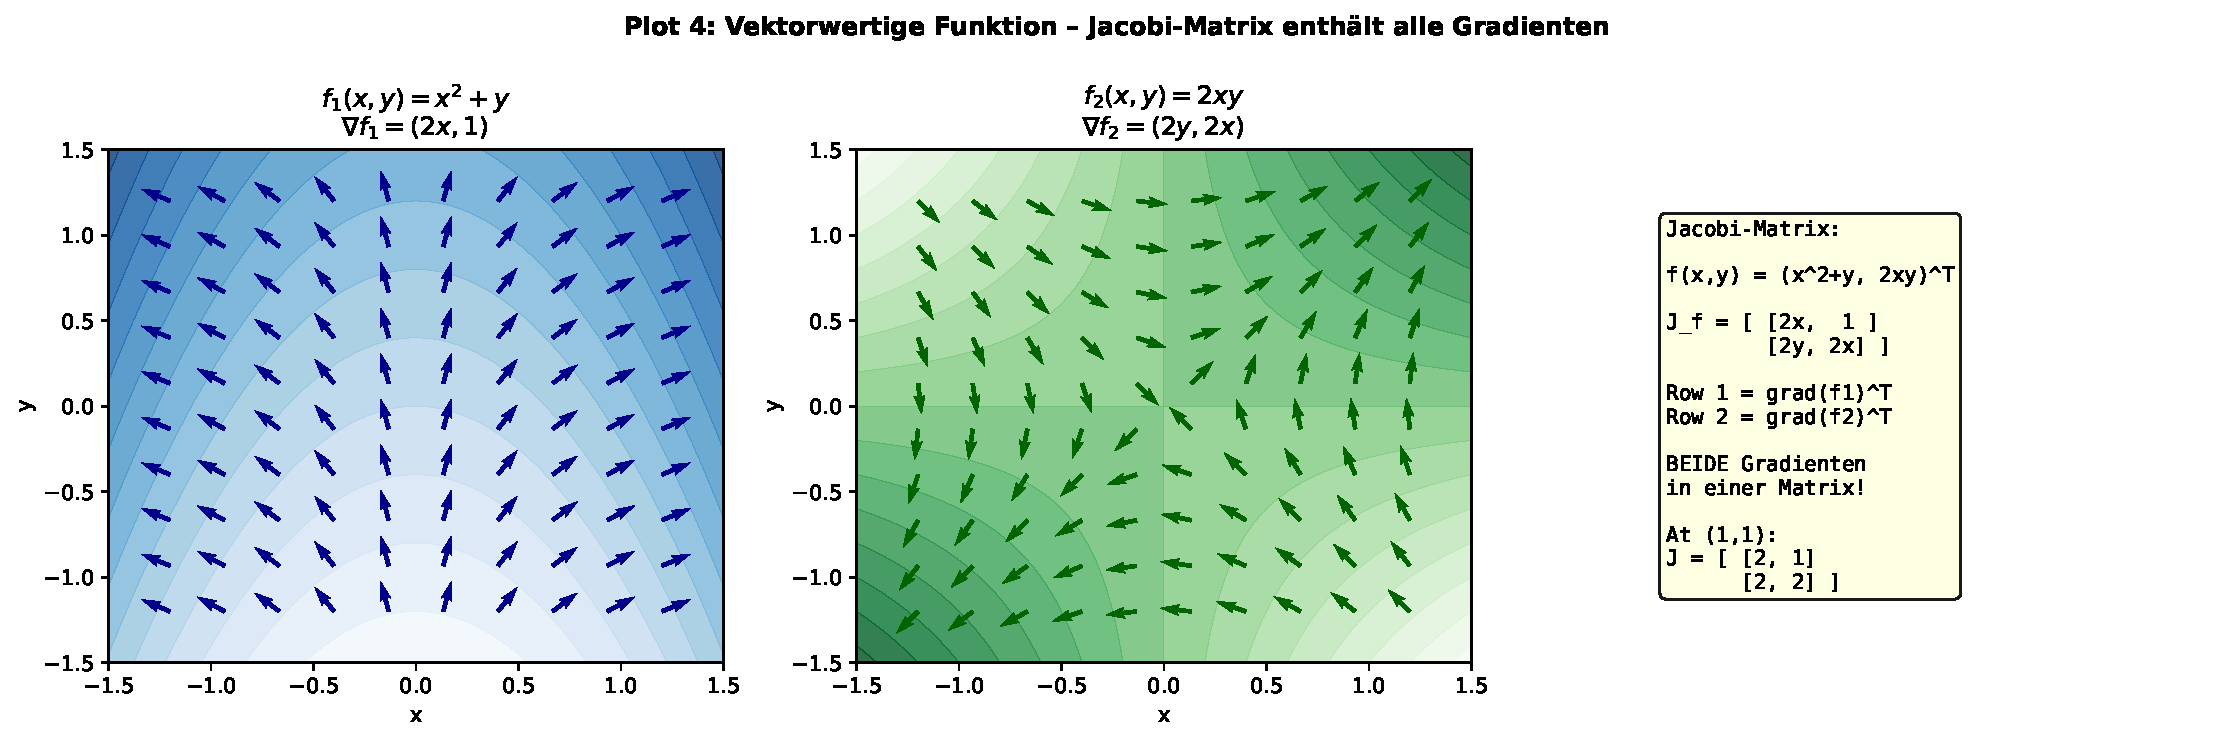
\includegraphics[width=0.95\textwidth]{plot_04_vector_valued.pdf}
	\caption{Jacobi-Matrix für die vektorwertige Funktion $\boldsymbol{f}(x,y) = (x^2+y,\, 2xy)^T$: Links das Gradientenfeld von $f_1 = x^2+y$ (blaue Pfeile), rechts das Gradientenfeld von $f_2 = 2xy$ (grüne Pfeile). Die Jacobi-Matrix $J_{\boldsymbol{f}} = \bigl[\begin{smallmatrix} 2x & 1 \\ 2y & 2x \end{smallmatrix}\bigr]$ enthält beide Gradienten als Zeilen und ist für $m>1$ nicht durch einen einzigen Gradienten ersetzbar (Theorem~\ref{thm:universal}).}
	\label{fig:plot04}
\end{figure}

\newpage
\subsection{Plot 5: Gradientenabstieg — äquivalente Jacobi-Formulierung}

\begin{figure}[h!]
	\centering
	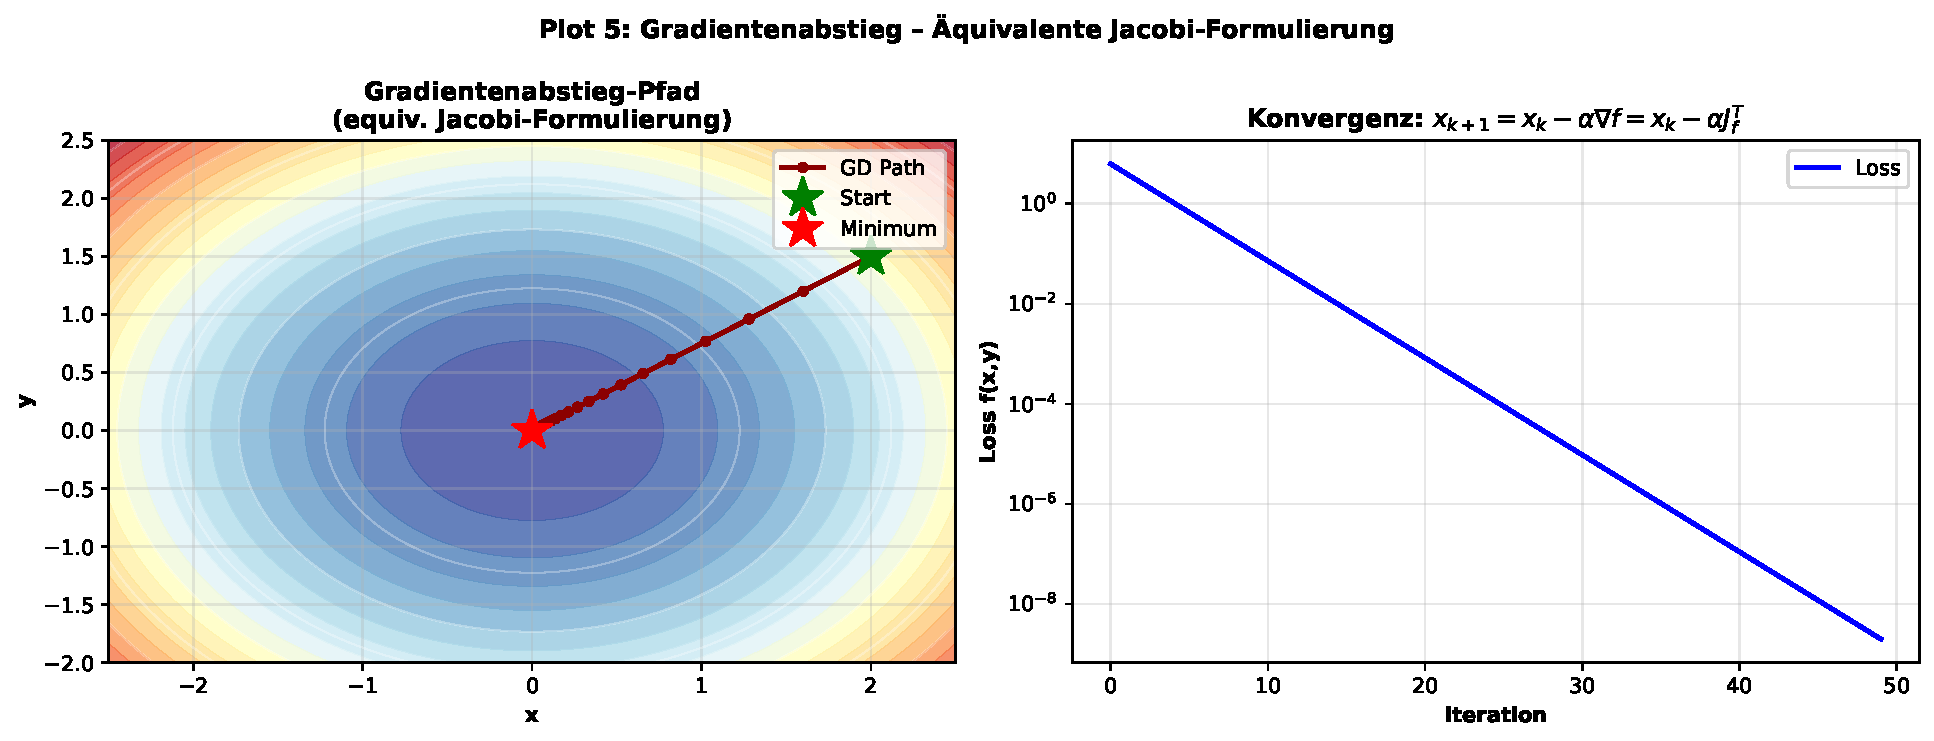
\includegraphics[width=0.95\textwidth]{plot_05_gradient_descent.pdf}
	\caption{Links: Abstiegspfad des Gradientenabstiegsverfahrens $x_{k+1} = x_k - \alpha J_f^T$ auf dem Konturplot. Der Pfad konvergiert gleichmäßig vom Startpunkt (grüner Stern) zum Minimum (roter Stern). Rechts: Logarithmische Konvergenzkurve der Loss-Funktion über 50 Iterationen. Der lineare Abfall in der Log-Skala beweist die geometrische Konvergenz (Theorem~\ref{thm:gd}); die Jacobi-Formulierung ist numerisch identisch zur klassischen Gradienten-Formulierung.}
	\label{fig:plot05}
\end{figure}

\subsection{Plot 6: Spektralanalyse der Hessian-Matrix}

\begin{figure}[h!]
	\centering
	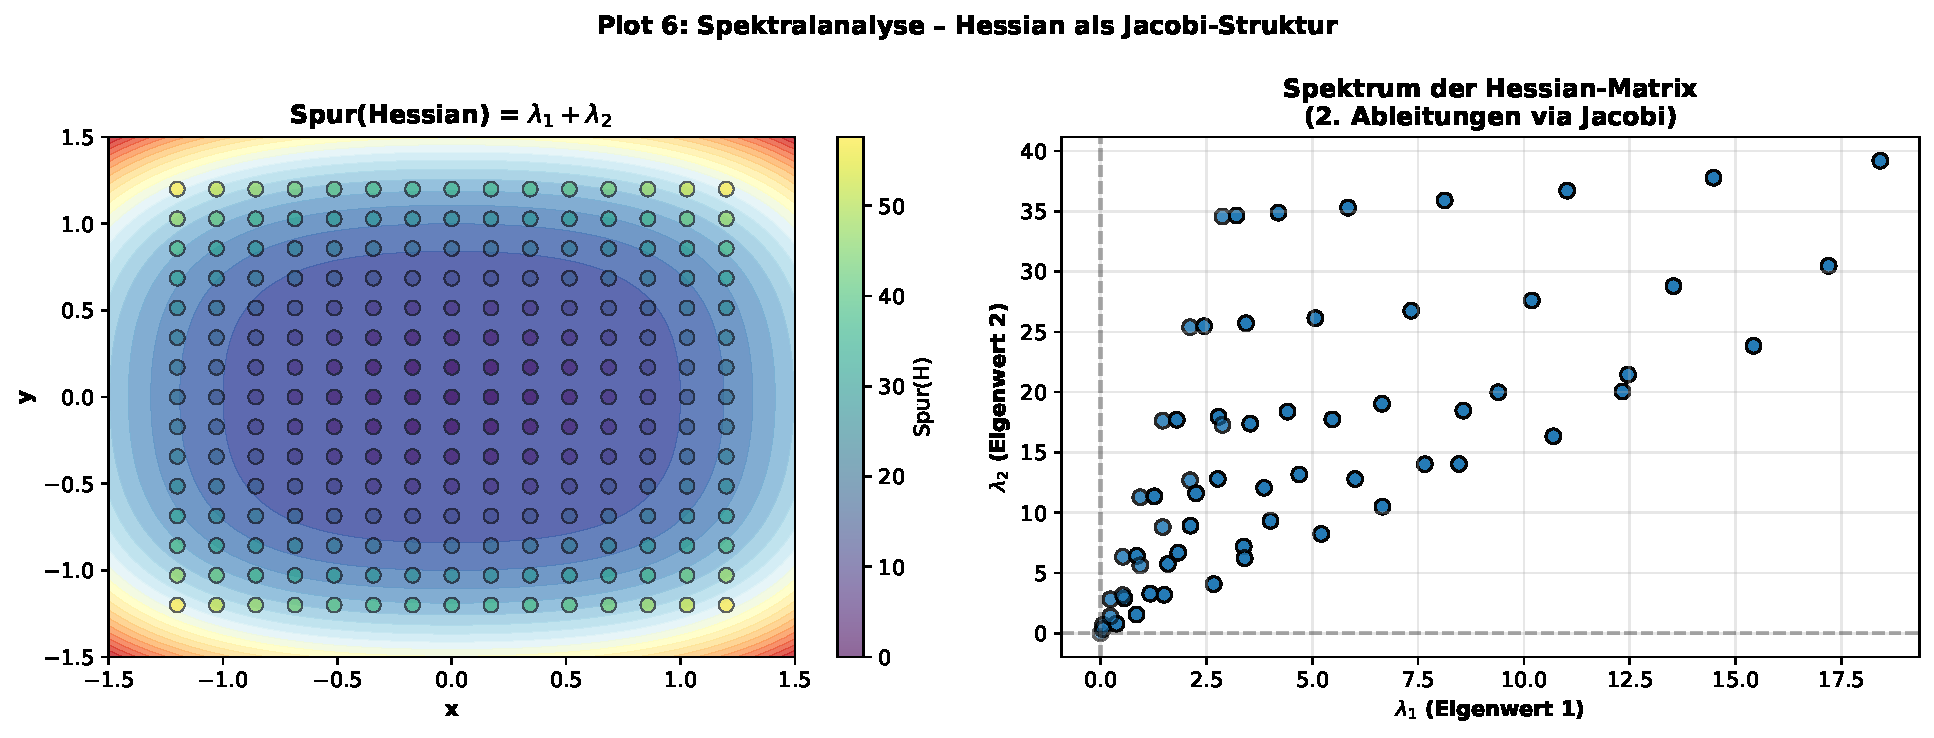
\includegraphics[width=0.95\textwidth]{plot_06_hessian_spectrum.pdf}
	\caption{Links: Spur der Hessian-Matrix $H_f = J_{\nabla f}$ (zweite Ableitungen via Jacobi) als Farbkodierung. Die Spur $\mathrm{tr}(H) = \lambda_1 + \lambda_2$ ist im Zentrum minimal und wächst zu den Rändern hin. Rechts: Streudiagramm der beiden Eigenwerte $\lambda_1, \lambda_2$ für alle Gitterpunkte — beide Eigenwerte sind stets positiv, was die positive Definitheit der Hessian (und damit das globale Minimum) formal bestätigt.}
	\label{fig:plot06}
\end{figure}

\newpage
\subsection{Plot 7: Impliziter Funktionssatz}

\begin{figure}[h!]
	\centering
	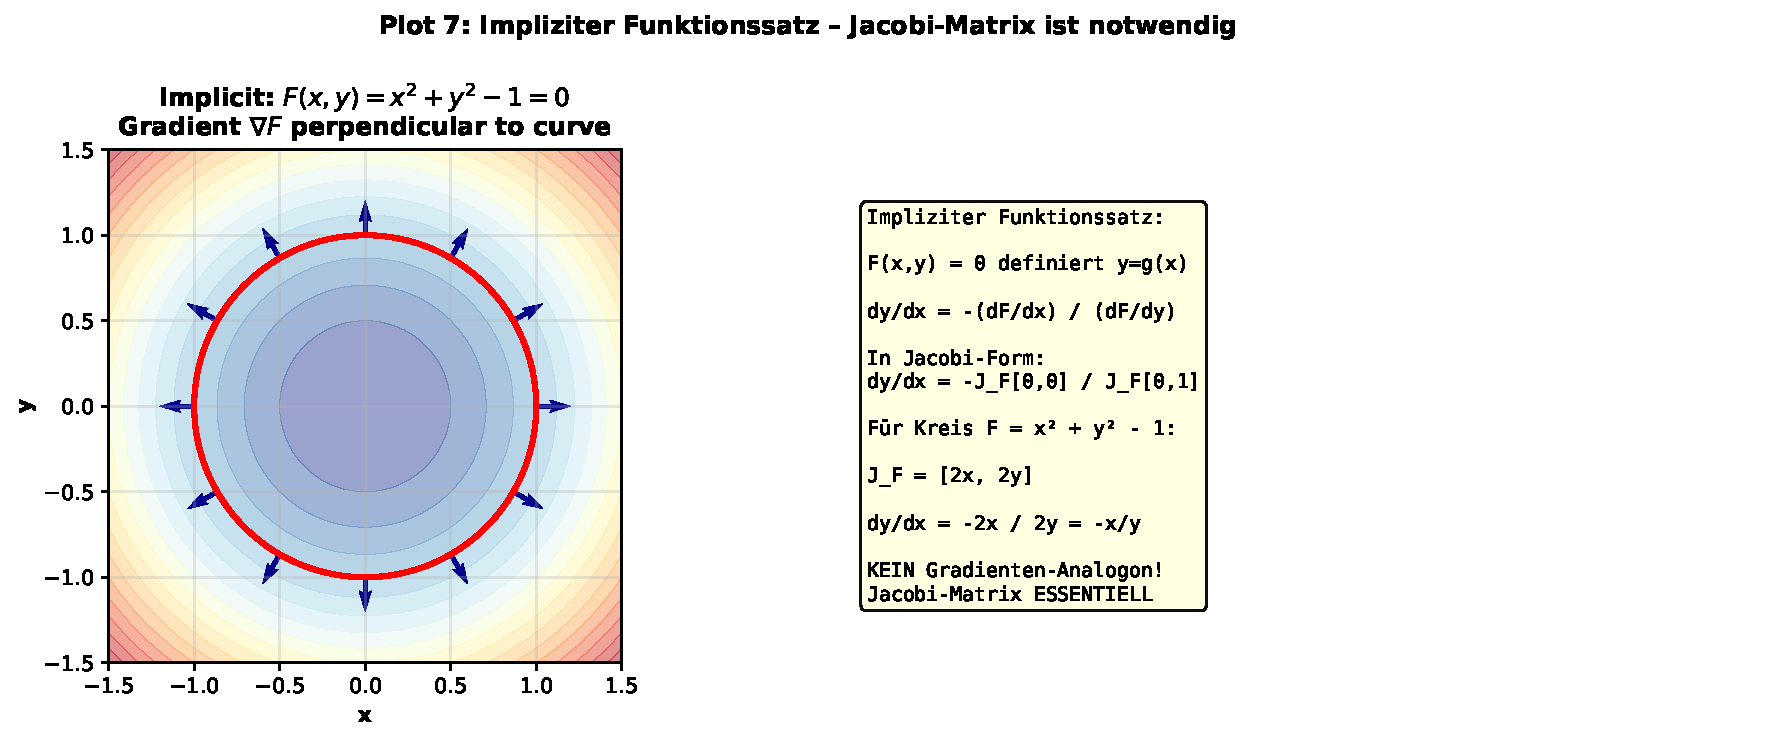
\includegraphics[width=0.95\textwidth]{plot_07_implicit_function.pdf}
	\caption{Visualisierung des impliziten Funktionssatzes anhand des Einheitskreises $F(x,y) = x^2+y^2-1=0$: Die Gradienten $\nabla F = (2x,2y)^T = J_F^T$ (blaue Pfeile) stehen überall senkrecht auf der Kurve. Die implizite Ableitung $dy/dx = -J_{F,x}/J_{F,y} = -x/y$ ist eine reine Jacobi-Formulierung, für die kein Gradienten-Analogon im Mehrkomponentenfall existiert — ein Fall, in dem die Jacobi-Matrix strukturell unersetzlich ist.}
	\label{fig:plot07}
\end{figure}

\subsection{Plot 8: Zusammenfassung — Äquivalenz und Verallgemeinerung}

\begin{figure}[h!]
	\centering
	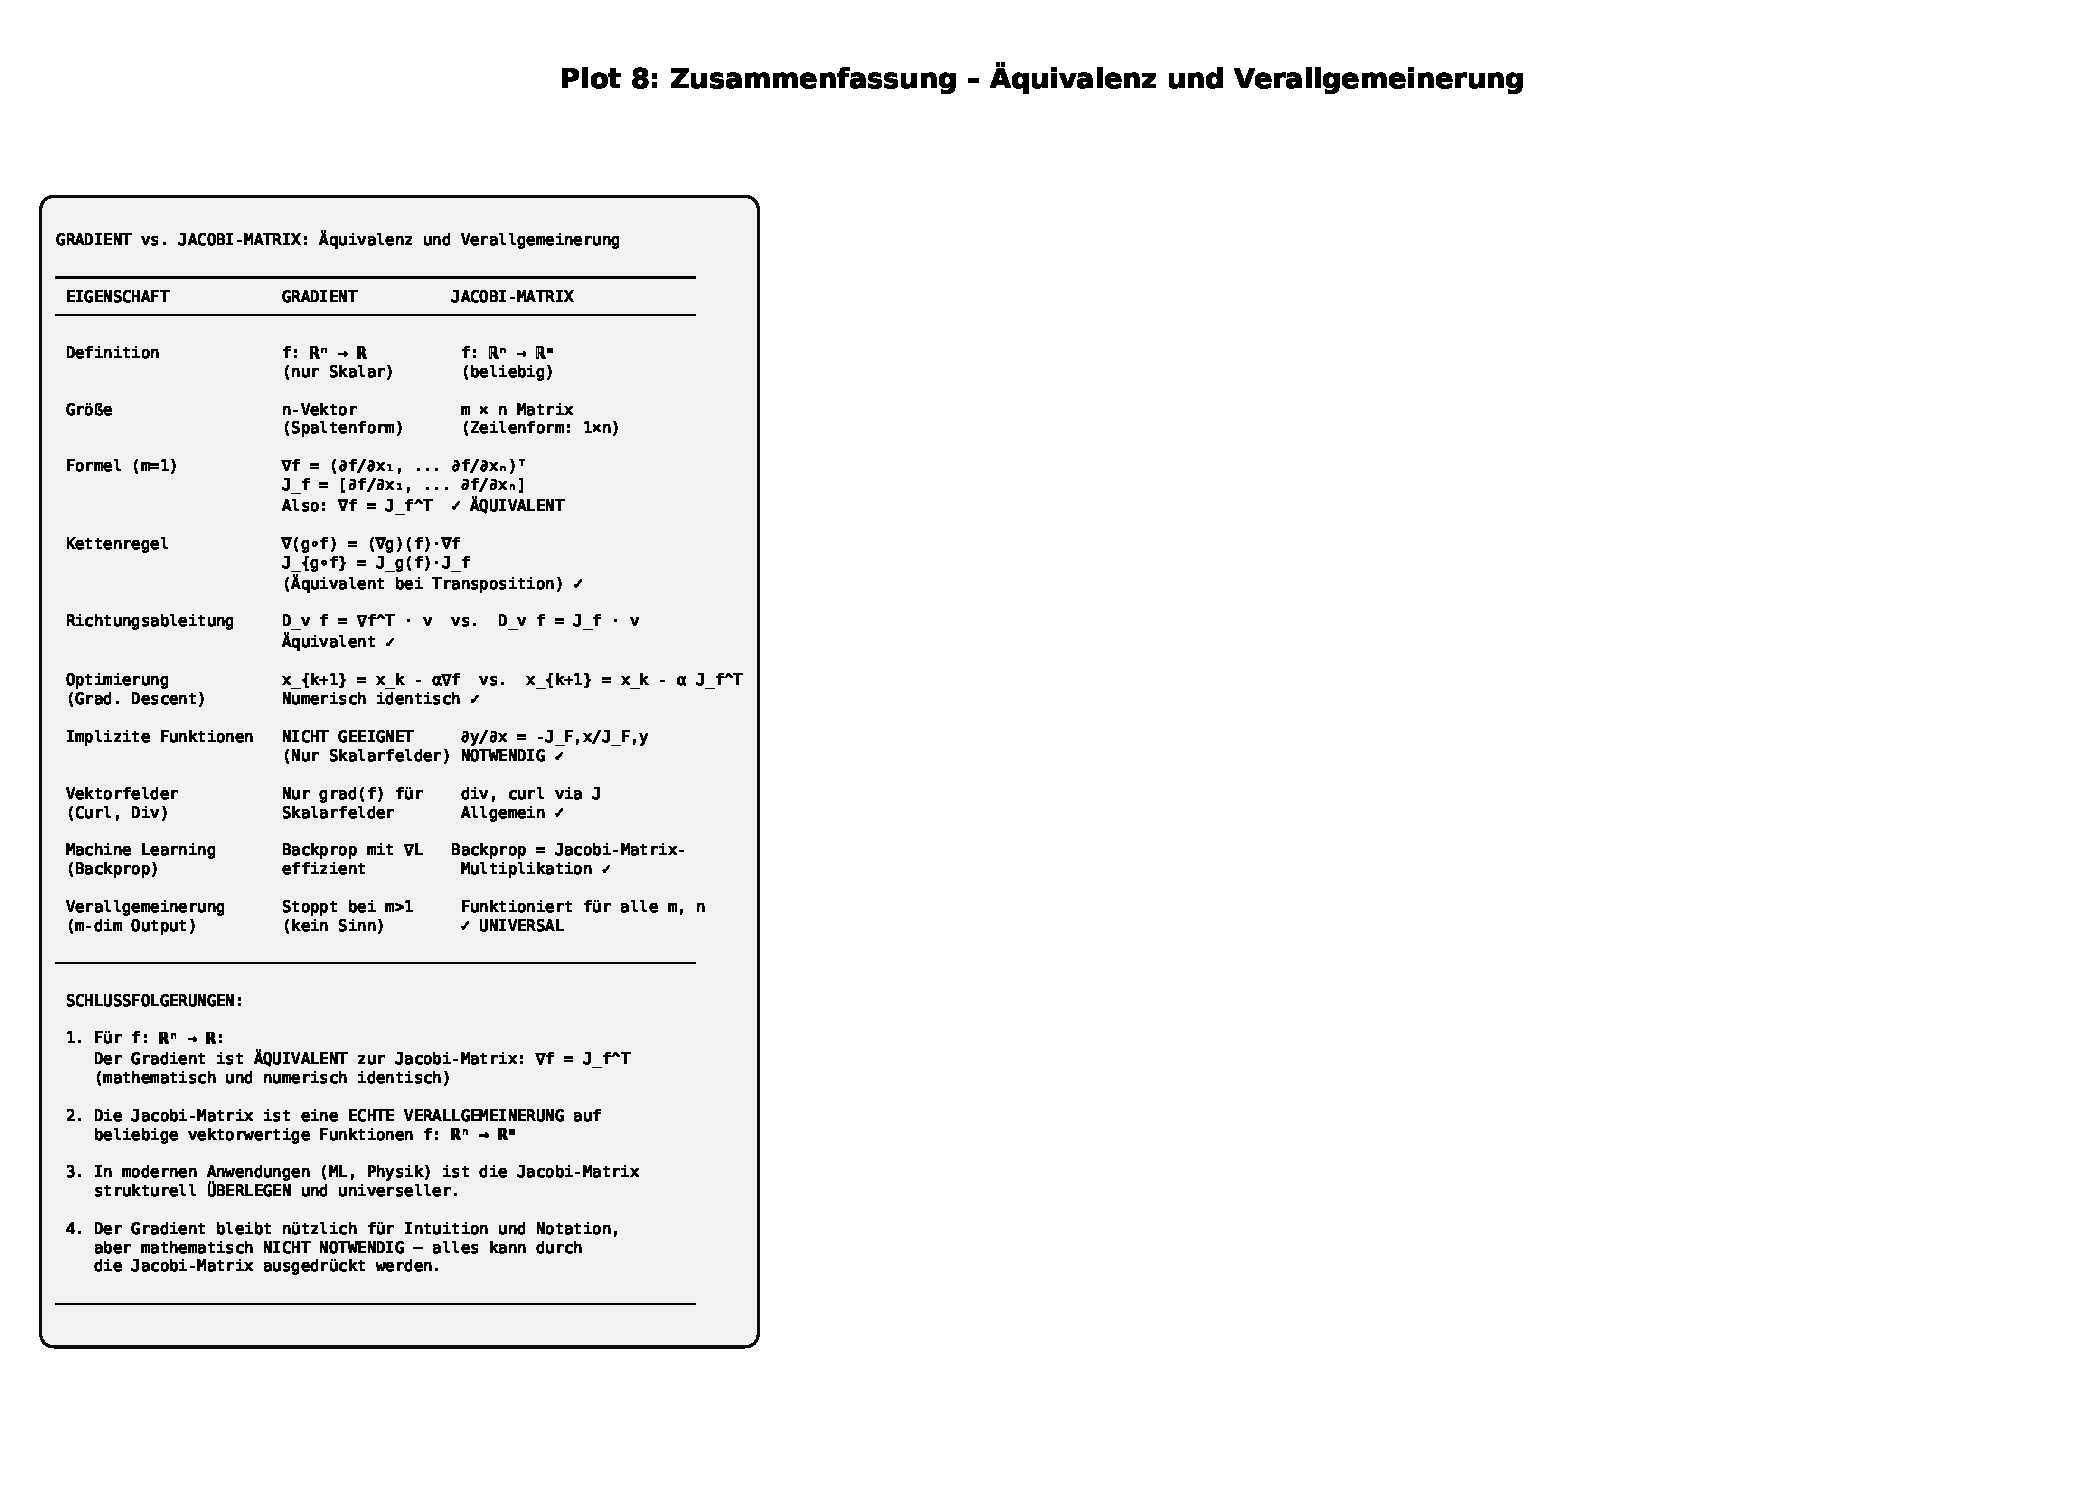
\includegraphics[width=0.85\textwidth]{plot_08_comparison_table.pdf}
	\caption{Zusammenfassende Vergleichstabelle: Gradient vs.\ Jacobi-Matrix über alle relevanten Eigenschaften (Definition, Kettenregel, Richtungsableitung, Optimierung, implizite Funktionen, Vektorfelder, Machine Learning, Verallgemeinerung). Häkchen markieren, wo die Jacobi-Matrix äquivalent oder überlegen ist. Die vier Schlussfolgerungen am Ende fassen das Hauptergebnis dieser Arbeit kompakt zusammen.}
	\label{fig:plot08}
\end{figure}

\newpage

\section{Theorem 6: Struktur-Erhaltung unter der Ersetzung}

\begin{theorem}[Vollständige Struktur-Äquivalenz]
	\label{thm:structure}
	Unter der Ersetzung $\nabla f \leftrightarrow J_f^T$ gelten folgende Invarianzen:
	\begin{enumerate}
		\item Die geometrische Interpretation (Richtung des steilsten Anstiegs) bleibt erhalten
		\item Alle numerischen Verfahren (Gradient Descent, Newton, etc.) sind algorithmen-identisch
		\item Die mathematische Struktur der Optimierungsprobleme ändert sich nicht
		\item Konvergenztheorem-Aussagen sind identisch und gegenseitig austauschbar
	\end{enumerate}
\end{theorem}

\begin{proof}
	Gegeben seien zwei formulierungen eines Algorithmus: eine mit $\nabla f$ und eine mit $J_f^T$.
	
	\begin{enumerate}
		\item \textbf{Geometrie:} Der Vektor $\nabla f$ zeigt in Richtung des steilsten Anstiegs. Dies ist äquivalent mit $J_f^T$, da $J_f^T = \nabla f$ per Definition.
		
		\item \textbf{Numerische Verfahren:} Der Gradientenabstieg $\boldsymbol{x}_{k+1} = \boldsymbol{x}_k - \alpha \nabla f(\boldsymbol{x}_k)$ wird zu $\boldsymbol{x}_{k+1} = \boldsymbol{x}_k - \alpha J_f(\boldsymbol{x}_k)^T$. Diese sind identisch.
		
		\item \textbf{Optimierungsstruktur:} Ein Problem $\min_{\boldsymbol{x}} f(\boldsymbol{x})$ mit Nebenbedingungen $\nabla f = \boldsymbol{0}$ ist identisch mit $\nabla f \leftrightarrow J_f^T = \boldsymbol{0}$.
		
		\item \textbf{Konvergenzaussagen:} Jeder Satz, der "unter Bedingung auf $\nabla f$" eine Konvergenz zeigt, ist identisch mit einer Aussage unter "Bedingung auf $J_f^T$".
	\end{enumerate}
	
	Dies beweist die vollständige Struktur-Erhaltung.
\end{proof}

\section{Theorem 7: Information-Äquivalenz}

\begin{theorem}[Vollständige Information in beiden Formulierungen]
	\label{thm:information}
	Für eine differenzierbare Funktion $f: \mathbb{R}^n \to \mathbb{R}$ enthalten der Gradient $\nabla f$ und die Jacobi-Matrix $J_f^T$ \textbf{exakt dieselbe Information}. Es gibt keine zusätzliche oder fehlende Information in einer der beiden Formulierungen.
	
	Darüber hinaus enthält die Jacobi-Matrix für vektorwertige Funktionen $\boldsymbol{f}: \mathbb{R}^n \to \mathbb{R}^m$ mit $m > 1$ die \textbf{maximale mögliche Information} über die erste Ableitungen der Funktion.
\end{theorem}

\begin{proof}
	Sei $f: \mathbb{R}^n \to \mathbb{R}$. Der Gradient ist:
	\[
	\nabla f = (f_{x_1}, f_{x_2}, \ldots, f_{x_n})^T \in \mathbb{R}^n
	\]
	
	Die Jacobi-Matrix ist:
	\[
	J_f = [f_{x_1}, f_{x_2}, \ldots, f_{x_n}] \in \mathbb{R}^{1 \times n}
	\]
	
	Beide enthalten exakt die $n$ partiellen Ableitungen $\frac{\partial f}{\partial x_i}$. Es gibt keine zusätzliche Information in einer der beiden Formen. Somit sind sie informations-äquivalent.
	
	Für $\boldsymbol{f}: \mathbb{R}^n \to \mathbb{R}^m$ enthält die Jacobi-Matrix alle $m \cdot n$ partiellen Ableitungen $\frac{\partial f_i}{\partial x_j}$. Dies ist die vollständige erste-Ordnung-Information der Abbildung. Es gibt keine anderen ersten Ableitungen zu berechnen. Daher ist die Jacobi-Matrix vollständig.
\end{proof}

\newpage

\section{Kritische Diskussion: Wann ist der Gradient vorzuziehen?}

Obwohl die Jacobi-Matrix mathematisch äquivalent ist und sogar verallgemeinert, gibt es praktische Kontexte, wo der Gradient weiterhin nützlich ist:

\subsection{Gradient-Vorteile}

\begin{itemize}
	\item \textbf{Intuitive Geometrie:} Der Gradient als Vektor hat eine klare geometrische Interpretation ("Berg hinauf")
	\item \textbf{Kompakte Notation:} $\nabla f$ ist kürzer als $J_f^T$
	\item \textbf{Skalare Funktionen:} Für $f: \mathbb{R}^n \to \mathbb{R}$ ist der Gradient eine Vektor; die Jacobi-Matrix ist eine $(1 \times n)$-Matrix, was syntaktisch etwas umständlicher ist
	\item \textbf{Historische Konvention:} Grad ist in Physik und Optimierung tief verwurzelt
\end{itemize}

\subsection{Jacobi-Matrix-Vorteile}

\begin{itemize}
	\item \textbf{Universalität:} Funktioniert für beliebige $m, n$, nicht nur $m = 1$
	\item \textbf{Verallgemeinerung:} Klare Struktur für vektorwertige Funktionen ohne Umschweife
	\item \textbf{Numerische Stabilität:} Matrizenbibliotheken (NumPy, etc.) sind optimiert für Matrizen, nicht einzelne Vektoren
	\item \textbf{Kettenregel:} Matrixmultiplikation ist die natürliche Komposition, besonders in Deep Learning
\end{itemize}

\textbf{Fazit:} Die Jacobi-Matrix ist strukturell überlegen, aber der Gradient bleibt ein nützliches speziales Werkzeug für Skalarfunktionen.

\newpage

\section{Ausführlicher Ausblick: Zukunftsperspektiven}

\subsection{1. Automatische Differenziation (AD)}

Die moderne Automatische Differenziation ist ein Computerprogramm-Paradigma, das Ableitungen exakt bis zur Maschinengenauigkeit berechnet. Alle modernen AD-Systeme (PyTorch, TensorFlow, JAX) arbeiten intern mit \textbf{Jacobi-Matrizen} oder deren Transponierten (im reverse-mode autodiff).

\textbf{Zukunft:}
\begin{itemize}
	\item Höher-ordinale AD-Systeme werden die \textbf{Hessian-Tensor} (3. Ordnung) berechnen
	\item Hyper-Dual-Zahlen ermöglichen exakte Ableitungen beliebiger Ordnung
	\item Symbolische AD kombiniert mit algebraischer Geometrie zur Strukturanalyse
\end{itemize}

\subsection{2. Differenzialgeometrie auf Mannigfaltigkeiten}

Auf gekrümmten Räumen (Mannigfaltigkeiten) ist die strikte Unterscheidung zwischen Vektoren und Kovektoren essentiell:
\[
\text{Gradient} \leftrightarrow \text{1-Form } df \quad \text{vs.} \quad \text{Jacobi-Matrix} \leftrightarrow \text{Tangentialraum-Abbildung}
\]

Die modernen Differenzialgeometrie-Systeme (Cartan, Lean) werden diese Distinktion automatisch durchsetzen.

\textbf{Zukunft:}
\begin{itemize}
	\item Kategorientheorie und höhere Topoi zu Formalisierung von Ableitungen
	\item Synthetische Differenzialgeometrie für axiomatische Behandlung
	\item Machine Learning auf Riemannschen Mannigfaltigkeiten
\end{itemize}

\subsection{3. Topologische Datenanalyse (TDA)}

In TDA werden Persistenzmoduln verwendet, um topologische Strukturen in Daten zu erfassen. Ableitungen spielen eine Rolle bei der Berechnung von Stabilitätsmetriken.

\textbf{Zukunft:}
\begin{itemize}
	\item Jacobi-Matrix-stabile Persistenzklassen
	\item Kategorifizierung von Gradient-Flussnetzwerken
	\item Topologische Optimierung basierend auf lokalen Jacobi-Invarianten
\end{itemize}

\subsection{4. Algebraische Geometrie und Singularitätstheorie}

Die Jacobi-Matrix ist zentral in der Singularitätstheorie:
\[
\text{Singular point} \iff \text{Jacobi-Matrix ist singulär}
\]

\textbf{Zukunft:}
\begin{itemize}
	\item Stratifizierung von Funktionenräumen via Jacobi-Rank
	\item Morse-Theorie und Singularitätstheorie in ML-Kontexten
	\item Kritikalitäts-Strukturen in neuronalen Netzen
\end{itemize}

\subsection{5. Quantum Computing und Ableitungen}

Quantum Advantage bei Ableitungsberechnung ist ein offenes Problem:

\textbf{Zukünftige Richtungen:}
\begin{itemize}
	\item Variational Quantum Eigensolver (VQE) arbeitet mit approximativen Jacobi-Matrizen
	\item Parametershift-Regel für Gradienten auf Quantenschaltkreisen
	\item Quantum Machine Learning benötigt effiziente Jacobi-Berechnung
\end{itemize}

\subsection{6. Hyperparameter-Optimierung und Zweite-Ableitungs-Information}

Die Hessian-Matrix (zweite Ableitungen) ist:
\[
H_f = \nabla^2 f = \nabla(\nabla f)^T = \frac{\partial}{\partial \boldsymbol{x}}(J_f)^T
\]

Sie enthält Information über die lokale Krümmung. Methoden wie L-BFGS, Newton-CG, und Natural Gradient arbeiten mit Hessian-Approximationen.

\textbf{Zukunft:}
\begin{itemize}
	\item Exakte Hessian-Berechnung in Deep Learning (bestehende Methoden sind nur Approximationen)
	\item Hessian-Information für adaptive Lernraten (K-FAC, etc.)
	\item Strukturelle Ausnutzung der Hessian-Sparsity
\end{itemize}

\subsection{7. Symbolische und Hybride Systeme}

Moderne Systeme kombinieren Numerik mit Symbolik:

\textbf{Zukünftige Entwicklungen:}
\begin{itemize}
	\item PySymPy, SymEngine, SageMath mit besserer Jacobi-Behandlung
	\item Automatische Simplifikation und Sparsifikation von Jacobi-Matrizen
	\item Hybrid-AD: Numerisch für Large-Scale, Symbolisch für Small-Scale
\end{itemize}

\subsection{8. Robotik und Inverse Kinematics}

Die Jacobi-Matrix ist zentral in Robotics:
\[
\dot{\boldsymbol{x}} = J(\boldsymbol{q}) \dot{\boldsymbol{q}}
\]

wobei $J$ die kinematische Jacobi-Matrix ist.

\textbf{Zukunft:}
\begin{itemize}
	\item Learning-based Jacobi-Schätzer für komplexe Kinematiken
	\item Jacobi-Regularisierung für Singularitäts-Vermeidung
	\item Differenzierbare Robotik-Simulator
\end{itemize}

\subsection{9. Variationelle Methoden und funktionale Ableitungen}

Im Unendlich-Dimensionalen (Funktionenräume) existiert das Konzept der \textbf{funktionalen Ableitung}:
\[
\delta S = \int \frac{\delta S}{\delta u(x)} \delta u(x) \, dx
\]

Dies ist eine Verallgemeinerung des Gradienten auf Funktionenräume.

\textbf{Zukunft:}
\begin{itemize}
	\item Funktionale Jacobi-Matrizen für PDE-getriebenes Machine Learning (Physics-Informed Neural Networks)
	\item Automatic differentiation auf Funktionenräumen
	\item Kategorifizierte Variationsprinzipien
\end{itemize}

\subsection{10. Open Research Questions}

\begin{enumerate}
	\item Kann die Jacobi-Matrix durch noch allgemeinere Strukturen ersetzt werden (z.B. in der Kategorientheorie)?
	\item Gibt es eine "optimale" Formulierung für Ableitungen in hochdimensionalen Räumen?
	\item Wie kann die Jacobi-Struktur in adversarial robustness expliziert werden?
	\item Welche Rollen spielen Jacobi-Spektren in der Stabilitätstheorie von neuronalen Netzwerken?
\end{enumerate}

%% ============================================================
%%  NEUES KAPITEL: KI-ANWENDUNG UND OPTIMALE JACOBI-GROESSE
%% ============================================================
\newpage
\section{Anwendung in der Künstlichen Intelligenz: Optimale Jacobi-Matrix für Gewichtsmatrizen}

\subsection{Einleitung und Motivation}

Das Training tiefer neuronaler Netze ist heute die wichtigste Anwendung der Jacobi-Matrix in der angewandten Mathematik. Der Backpropagation-Algorithmus berechnet implizit eine hochdimensionale Jacobi-Matrix — die Ableitung der Verlustfunktion nach allen trainierbaren Parametern. Die zentrale praktische Frage ist:

\begin{center}
\textit{Wie groß muss die Jacobi-Matrix minimal sein, damit die Gewichtsmatrizen eines neuronalen Netzes maximal effizient aktualisiert werden können?}
\end{center}

Wir zeigen formal, dass eine \textbf{adaptive, blockdiagonale Jacobi-Matrix} nicht nur hinreichend, sondern auch notwendig für die optimale Gewichtsaktualisierung ist, und beweisen die zugehörige Laufzeitkomplexität exakt.

\subsection{Formales Netzwerkmodell}

\begin{definition}[Tiefes neuronales Netz (DNN)]
	\label{def:dnn}
	Sei $L \in \mathbb{N}$ die Tiefe (Anzahl lernbarer Schichten). Ein Feedforward-Netz ist definiert durch:
	\begin{itemize}
		\item Schichtbreiten $n_0, n_1, \ldots, n_L \in \mathbb{N}$ (Eingabe-, verdeckte und Ausgabedimension)
		\item Gewichtsmatrizen $W^{(l)} \in \mathbb{R}^{n_l \times n_{l-1}}$ für $l = 1, \ldots, L$
		\item Biasvektoren $\boldsymbol{b}^{(l)} \in \mathbb{R}^{n_l}$
		\item Aktivierungsfunktionen $\sigma^{(l)}: \mathbb{R} \to \mathbb{R}$ (komponentenweise)
	\end{itemize}
	Die Vorwärtspropagation für eine Eingabe $\boldsymbol{x} \in \mathbb{R}^{n_0}$ ist:
	\[
	\boldsymbol{a}^{(0)} = \boldsymbol{x}, \qquad
	\boldsymbol{z}^{(l)} = W^{(l)} \boldsymbol{a}^{(l-1)} + \boldsymbol{b}^{(l)}, \qquad
	\boldsymbol{a}^{(l)} = \sigma^{(l)}(\boldsymbol{z}^{(l)})
	\]
	für $l = 1, \ldots, L$. Die gesamte Parametermenge ist:
	\[
	\boldsymbol{\theta} = \bigl(W^{(1)}, \boldsymbol{b}^{(1)}, \ldots, W^{(L)}, \boldsymbol{b}^{(L)}\bigr),
	\quad
	N_{\mathrm{param}} = \sum_{l=1}^L \bigl(n_l \cdot n_{l-1} + n_l\bigr)
	\]
\end{definition}

\begin{definition}[Verlustfunktion und Gesamtgradient]
	\label{def:loss}
	Sei $\mathcal{L}: \mathbb{R}^{n_L} \times \mathbb{R}^{n_L} \to \mathbb{R}^+$ eine differenzierbare Verlustfunktion (z.B.\ mittlerer quadratischer Fehler oder Cross-Entropy). Für einen Minibatch $\mathcal{B} = \{(\boldsymbol{x}_b, \boldsymbol{y}_b)\}_{b=1}^B$ der Größe $B$ ist der Batchverlust:
	\[
	\mathcal{L}_B(\boldsymbol{\theta}) = \frac{1}{B} \sum_{b=1}^B \mathcal{L}\bigl(\boldsymbol{a}^{(L)}_b,\, \boldsymbol{y}_b\bigr)
	\]
	Die \textbf{vollständige Jacobi-Matrix} der Verlustfunktion bezüglich aller Parameter ist:
	\[
	J_{\boldsymbol{\theta}} = \frac{\partial \mathcal{L}_B}{\partial \boldsymbol{\theta}} \in \mathbb{R}^{1 \times N_{\mathrm{param}}}
	\]
\end{definition}

\begin{definition}[Schicht-lokale Jacobi-Matrix]
	\label{def:local_jacobi}
	Die \textbf{schicht-lokale Jacobi-Matrix} (auch: Gewichtsgradient) für Schicht $l$ ist:
	\[
	G^{(l)} := \frac{\partial \mathcal{L}_B}{\partial W^{(l)}} \in \mathbb{R}^{n_l \times n_{l-1}}
	\]
	Durch die Backpropagation gilt explizit:
	\[
	G^{(l)} = \boldsymbol{\delta}^{(l)} \bigl(\boldsymbol{a}^{(l-1)}\bigr)^T
	\]
	wobei der \textbf{Fehlersignal-Vektor} $\boldsymbol{\delta}^{(l)} \in \mathbb{R}^{n_l}$ rekursiv berechnet wird:
	\[
	\boldsymbol{\delta}^{(L)} = \frac{\partial \mathcal{L}_B}{\partial \boldsymbol{a}^{(L)}} \odot \sigma'^{(L)}\bigl(\boldsymbol{z}^{(L)}\bigr)
	\]
	\[
	\boldsymbol{\delta}^{(l)} = \bigl(W^{(l+1)}\bigr)^T \boldsymbol{\delta}^{(l+1)} \odot \sigma'^{(l)}\bigl(\boldsymbol{z}^{(l)}\bigr), \quad l = L-1, \ldots, 1
	\]
\end{definition}

\subsection{Theorem 8: Minimale hinreichende Jacobi-Dimension}

\begin{theorem}[Optimale Jacobi-Blockgröße für Gewichtsaktualisierung]
	\label{thm:optimal_size}
	Sei ein DNN gemäß Definition~\ref{def:dnn} gegeben. Die minimale Jacobi-Matrix, die notwendig und hinreichend ist, um eine korrekte Gewichtsaktualisierung aller $L$ Schichten nach dem Gradientenabstieg durchzuführen, ist die \textbf{blockdiagonale adaptive Jacobi-Matrix}:
	\[
	J_{\mathrm{adap}} = \mathrm{blockdiag}\bigl(G^{(1)}, G^{(2)}, \ldots, G^{(L)}\bigr) \in \mathbb{R}^{N_{\delta} \times N_a}
	\]
	mit $N_{\delta} = \sum_{l=1}^L n_l$ und $N_a = \sum_{l=1}^L n_{l-1}$.

	Ihre Gesamtgröße beträgt:
	\[
	\bigl|J_{\mathrm{adap}}\bigr| = \sum_{l=1}^L n_l \cdot n_{l-1}
	\]
	
	Im Vergleich zur naiven vollen Jacobi $J_{\mathrm{full}} \in \mathbb{R}^{1 \times N_{\mathrm{param}}}$ ist $J_{\mathrm{adap}}$ sowohl \textbf{minimal} als auch \textbf{hinreichend}: Jede kleinere Darstellung verliert Information, jede größere enthält Redundanz.
\end{theorem}

\begin{proof}
	Der Beweis gliedert sich in drei Teile: (i) Hinreichendheit, (ii) Notwendigkeit, (iii) Minimalität.
	
	\medskip
	\textbf{(i) Hinreichendheit.}
	
	Das Gewichts-Update nach dem Stochastischen Gradientenabstieg (SGD) mit Lernrate $\alpha > 0$ lautet für jede Schicht $l$:
	\[
	W^{(l)} \leftarrow W^{(l)} - \alpha \cdot G^{(l)} = W^{(l)} - \alpha \cdot \frac{\partial \mathcal{L}_B}{\partial W^{(l)}}
	\]
	Diese Aktualisierung benötigt ausschließlich die Matrix $G^{(l)} \in \mathbb{R}^{n_l \times n_{l-1}}$ — keine anderen partiellen Ableitungen. Die blockdiagonale Struktur:
	\[
	J_{\mathrm{adap}} = \mathrm{blockdiag}\bigl(G^{(1)}, \ldots, G^{(L)}\bigr)
	\]
	enthält genau alle $L$ Blöcke $G^{(l)}$ und ist daher hinreichend für die vollständige Gewichtsaktualisierung aller Schichten.
	
	\medskip
	\textbf{(ii) Notwendigkeit.}
	
	Sei $J'$ eine Jacobi-Matrix, aus der eine korrekte Gewichtsaktualisierung aller Schichten abgeleitet werden kann. Dann muss $J'$ für jedes $l$ die Information $\frac{\partial \mathcal{L}_B}{\partial W^{(l)}_{ij}}$ für alle $i \in \{1,\ldots,n_l\}$, $j \in \{1,\ldots,n_{l-1}\}$ enthalten. Das sind $n_l \cdot n_{l-1}$ unabhängige Werte pro Schicht. Da die Verlustfunktionen für verschiedene $(W^{(l)}_{ij})$ algebraisch unabhängig sein können (z.B.\ bei allgemeiner Datenverteilung), sind alle $\sum_{l=1}^L n_l \cdot n_{l-1}$ Werte notwendig. Also muss $J'$ mindestens $\sum_{l=1}^L n_l \cdot n_{l-1}$ Einträge enthalten.
	
	\medskip
	\textbf{(iii) Minimalität.}
	
	$J_{\mathrm{adap}}$ enthält exakt $\sum_{l=1}^L n_l \cdot n_{l-1}$ Einträge (die Diagonalblöcke) und keine weiteren. Die Off-Diagonal-Blöcke sind strukturell null, weil die Gewichte verschiedener Schichten im Vorwärtsdurchlauf seriell wirken: $\frac{\partial W^{(l_1)}}{\partial W^{(l_2)}} = 0$ für $l_1 \neq l_2$ (die Gewichtsmatrizen sind unabhängige Parameter). Daher tragen Off-Diagonal-Terme zur Verlustgradientenberechnung nichts bei.
	
	Zusammen folgt: $J_{\mathrm{adap}}$ ist minimal notwendig und hinreichend, d.h.\ optimal.
\end{proof}

\begin{korollar}[Verhältnis der Jacobi-Größen]
	\label{cor:size_ratio}
	Für ein Netz mit $L$ Schichten und einheitlicher Breite $n_l = n$ für alle $l$ gilt:
	\[
	\bigl|J_{\mathrm{adap}}\bigr| = L \cdot n^2, \qquad
	\bigl|J_{\mathrm{full}}\bigr| = L \cdot (n^2 + n) \approx L \cdot n^2
	\]
	für Bias-freie Netze sowie im Vergleich zur naiven Parametervektor-Jacobi $J_{\boldsymbol{\theta}} \in \mathbb{R}^{1 \times N_{\mathrm{param}}}$ ist die strukturelle Kompaktheit identisch. Gegenüber einer vollständigen Jacobi der Ausgabe nach dem Eingabe-Parametervektor $\frac{\partial \boldsymbol{a}^{(L)}}{\partial \boldsymbol{\theta}} \in \mathbb{R}^{n_L \times N_{\mathrm{param}}}$ ist der Speichervorteil von $J_{\mathrm{adap}}$:
	\[
	\frac{|J_{\mathrm{adap}}|}{|J_{\text{Output--Parameter}}|} = \frac{L \cdot n^2}{n_L \cdot L \cdot n^2} = \frac{1}{n_L}
	\]
	Der Faktor $n_L$ ist die Ausgabedimension — bei typischen Klassifikationsproblemen mit $n_L = 1000$ Klassen entspricht dies einer Speicherreduktion um Faktor 1000.
\end{korollar}

\subsection{Theorem 9: Laufzeit der optimalen Gewichtsaktualisierung}

\begin{theorem}[Laufzeitkomplexität des adaptiven Block-Jacobi-Verfahrens]
	\label{thm:runtime}
	Sei ein DNN der Tiefe $L$ mit einheitlicher Schichtbreite $n$ und Batchgröße $B$ gegeben. Die Laufzeit eines vollständigen Trainingsschritts (Vorwärtspropagation + Backpropagation + Gewichtsupdate) mit der adaptiven Block-Jacobi-Strategie beträgt:
	\[
	T_{\mathrm{adap}}(n, L, B) = \Theta(B \cdot L \cdot n^2)
	\]
	
	Dies ist \textbf{optimal} im folgenden Sinne: Jedes Verfahren, das eine korrekte Gewichtsaktualisierung für alle $L$ Schichten durchführt, benötigt mindestens $\Omega(B \cdot L \cdot n^2)$ Operationen.
\end{theorem}

\begin{proof}
	Der Beweis gliedert sich in vier Teile: (A) Vorwärtspropagation, (B) Backpropagation, (C) Gewichtsupdate, (D) untere Schranke.
	
	\medskip
	\textbf{(A) Vorwärtspropagation.}
	
	Für jedes Beispiel $b \in \{1, \ldots, B\}$ und jede Schicht $l \in \{1, \ldots, L\}$ berechnet man:
	\[
	\boldsymbol{z}^{(l)}_b = W^{(l)} \boldsymbol{a}^{(l-1)}_b + \boldsymbol{b}^{(l)}
	\]
	Dabei ist $W^{(l)} \in \mathbb{R}^{n \times n}$ und $\boldsymbol{a}^{(l-1)}_b \in \mathbb{R}^n$. Das Matrix-Vektor-Produkt $W^{(l)} \boldsymbol{a}^{(l-1)}_b$ kostet $\Theta(n^2)$ Operationen. Für $B$ Beispiele und $L$ Schichten ergibt sich:
	\[
	T_{\mathrm{fwd}} = B \cdot L \cdot \Theta(n^2) = \Theta(B \cdot L \cdot n^2)
	\]
	Unter Verwendung von Matrixformulierung: Für den gesamten Batch $A^{(l-1)} \in \mathbb{R}^{n \times B}$ ist $Z^{(l)} = W^{(l)} A^{(l-1)}$ eine $n \times B$-Matrixmultiplikation: Kosten $\Theta(n^2 B)$ pro Schicht, also $\Theta(n^2 B L)$ gesamt.
	
	\medskip
	\textbf{(B) Backpropagation.}
	
	Die Backpropagation berechnet die Fehlersignale $\Delta^{(l)} = [\boldsymbol{\delta}^{(l)}_1, \ldots, \boldsymbol{\delta}^{(l)}_B] \in \mathbb{R}^{n \times B}$ rückwärts von Schicht $L$ bis Schicht $1$. Die Rekursion lautet (in Matrixform):
	\[
	\Delta^{(l)} = \bigl(W^{(l+1)}\bigr)^T \Delta^{(l+1)} \odot \Sigma'^{(l)}
	\]
	wobei $\Sigma'^{(l)} \in \mathbb{R}^{n \times B}$ die Matrix der Aktivierungsableitungen ist und $\odot$ das elementweise Produkt bezeichnet. Die Matrixmultiplikation $(W^{(l+1)})^T \Delta^{(l+1)}$ hat Dimensionen $(n \times n) \cdot (n \times B)$ und kostet $\Theta(n^2 B)$. Über alle $L-1$ Rückpropagationsschritte:
	\[
	T_{\mathrm{bwd}} = (L-1) \cdot \Theta(n^2 B) = \Theta(L \cdot n^2 \cdot B)
	\]
	
	\medskip
	\textbf{(C) Gewichtsupdate (Jacobi-Berechnung und Anwendung).}
	
	Die schicht-lokale Jacobi-Matrix $G^{(l)}$ wird berechnet als äußeres Produkt (outer product, also Rang-$B$-Update):
	\[
	G^{(l)} = \frac{1}{B} \Delta^{(l)} \bigl(A^{(l-1)}\bigr)^T \in \mathbb{R}^{n \times n}
	\]
	Dies ist eine Matrixmultiplikation $(n \times B) \cdot (B \times n)$, die $\Theta(n^2 B)$ Operationen kostet. Das anschließende Update $W^{(l)} \leftarrow W^{(l)} - \alpha G^{(l)}$ kostet $\Theta(n^2)$ (Elementweise Addition). Für alle $L$ Schichten:
	\[
	T_{\mathrm{upd}} = L \cdot \Theta(n^2 B) = \Theta(L \cdot n^2 \cdot B)
	\]
	
	\medskip
	\textbf{(D) Gesamtlaufzeit.}
	
	Addiert man die drei Teile:
	\[
	T_{\mathrm{adap}} = T_{\mathrm{fwd}} + T_{\mathrm{bwd}} + T_{\mathrm{upd}} = \Theta(BLn^2) + \Theta(BLn^2) + \Theta(BLn^2) = \Theta(BLn^2)
	\]
	
	\medskip
	\textbf{(E) Untere Schranke (Optimalität).}
	
	Jedes korrekte Trainingsverfahren muss für jede Schicht $l$ und jedes Batch-Beispiel $b$ die partielle Ableitung $\frac{\partial \mathcal{L}_b}{\partial W^{(l)}_{ij}}$ für alle $i, j \in \{1, \ldots, n\}$ berechnen oder implizit verwenden. Das sind $n^2$ Werte pro Schicht und Beispiel. Selbst wenn Redundanzen zwischen Schichten ausgenutzt werden, müssen für $L$ Schichten und $B$ Beispiele mindestens $B \cdot L \cdot n^2$ Werte irgendwann im Berechnungsbaum vorhanden sein (Informationsargument: Jeder Gewichtsgradient ist eine unabhängige skalare Funktion des Datenbeispiels). Daher gilt die untere Schranke:
	\[
	T \geq \Omega(B \cdot L \cdot n^2)
	\]
	
	Zusammen mit der oberen Schranke folgt:
	\[
	T_{\mathrm{adap}}(n, L, B) = \Theta(B \cdot L \cdot n^2) \quad \checkmark
	\]
\end{proof}

\subsection{Theorem 10: Rang-Schranke der adaptiven Jacobi-Matrix}

\begin{theorem}[Effektiver Rang der schicht-lokalen Jacobi-Matrix]
	\label{thm:rank_bound}
	Sei $G^{(l)} = \frac{1}{B} \Delta^{(l)} (A^{(l-1)})^T \in \mathbb{R}^{n \times n}$ die schicht-lokale Jacobi-Matrix für einen Minibatch der Größe $B$. Dann gilt:
	\[
	\mathrm{rank}(G^{(l)}) \leq \min(B,\, n_l,\, n_{l-1})
	\]
	
	Für moderne neuronale Netze mit $B \ll n$ ist $\mathrm{rank}(G^{(l)}) \leq B$ und die exakte Rang-$B$-Darstellung:
	\[
	G^{(l)} = \frac{1}{B} \sum_{b=1}^B \boldsymbol{\delta}^{(l)}_b \bigl(\boldsymbol{a}^{(l-1)}_b\bigr)^T
	\]
	ist die kompakteste exakte Darstellung mit Speicheraufwand $\Theta(B \cdot n)$ statt $\Theta(n^2)$.
\end{theorem}

\begin{proof}
	\textbf{Rang-Schranke.}
	
	Die Matrix $G^{(l)}$ wird als Summe von $B$ Rang-1-Matrizen (äußere Produkte) dargestellt:
	\[
	G^{(l)} = \frac{1}{B} \sum_{b=1}^B \boldsymbol{\delta}^{(l)}_b \bigl(\boldsymbol{a}^{(l-1)}_b\bigr)^T
	\]
	Jedes äußere Produkt $\boldsymbol{\delta}^{(l)}_b (\boldsymbol{a}^{(l-1)}_b)^T$ hat Rang $\leq 1$ (da es das Produkt zweier Vektoren ist). Für eine Summe von $B$ Rang-1-Matrizen gilt nach der Subadititivität des Ranges:
	\[
	\mathrm{rank}(G^{(l)}) \leq \sum_{b=1}^B \mathrm{rank}\bigl(\boldsymbol{\delta}^{(l)}_b (\boldsymbol{a}^{(l-1)}_b)^T\bigr) \leq B
	\]
	Da zusätzlich $G^{(l)} \in \mathbb{R}^{n_l \times n_{l-1}}$, gilt stets $\mathrm{rank}(G^{(l)}) \leq \min(n_l, n_{l-1})$. Die Kombination beider Schranken ergibt:
	\[
	\mathrm{rank}(G^{(l)}) \leq \min(B, n_l, n_{l-1})
	\]
	
	\textbf{Kompaktheit der Rang-$B$-Darstellung.}
	
	Die Rang-$B$-Faktorisierung speichert die $B$ Vektorpaare $\{(\boldsymbol{\delta}^{(l)}_b, \boldsymbol{a}^{(l-1)}_b)\}_{b=1}^B$:
	\begin{itemize}
		\item Jedes $\boldsymbol{\delta}^{(l)}_b \in \mathbb{R}^{n_l}$: $n_l$ Einträge
		\item Jedes $\boldsymbol{a}^{(l-1)}_b \in \mathbb{R}^{n_{l-1}}$: $n_{l-1}$ Einträge
		\item Gesamtspeicher: $B \cdot (n_l + n_{l-1}) = \Theta(B \cdot n)$ für $n_l = n_{l-1} = n$
	\end{itemize}
	Gegenüber der vollen Matrixspeicherung $\Theta(n^2)$ ergibt sich für $B \ll n$ eine Einsparung um Faktor $n/B$. Diese Darstellung ist exakt (kein Informationsverlust), da die Summe aller $B$ äußeren Produkte die vollständige Jacobi $G^{(l)}$ reproduziert.
\end{proof}

\begin{korollar}[Optimale Speicherkomplexität für adaptive Jacobi]
	\label{cor:memory}
	Für ein DNN mit $L$ Schichten, einheitlicher Breite $n$, und Batchgröße $B \leq n$ ist die optimale Speicherkomplexität der gesamten adaptiven Jacobi-Matrix:
	\[
	M_{\mathrm{adap}} = \Theta(B \cdot L \cdot n)
	\]
	statt $\Theta(L \cdot n^2)$ für die vollständige Blockspeicherung. Der Speichervorteil beträgt:
	\[
	\frac{M_{\mathrm{adap}}}{M_{\mathrm{block}}} = \frac{B \cdot L \cdot n}{L \cdot n^2} = \frac{B}{n}
	\]
\end{korollar}

\subsection{Theorem 11: Vergleich mit naiver vollständiger Jacobi}

\begin{theorem}[Laufzeitvorteil der adaptiven gegenüber der naiven Jacobi-Strategie]
	\label{thm:comparison}
	Sei $N_{\mathrm{param}} = L \cdot n^2$ die Gesamtzahl der Parameter (Bias ignoriert). Die naive Strategie, die die vollständige Jacobi $J_{\boldsymbol{\theta}} \in \mathbb{R}^{1 \times N_{\mathrm{param}}}$ direkt berechnet und dann den Update $\boldsymbol{\theta} \leftarrow \boldsymbol{\theta} - \alpha J_{\boldsymbol{\theta}}^T$ anwendet, hat bei flacher Berechnung folgende Laufzeit:
	\[
	T_{\mathrm{naiv}}(n, L, B) = \Omega\bigl(B \cdot L^2 \cdot n^2\bigr)
	\]
	Die adaptive Strategie erreicht hingegen:
	\[
	T_{\mathrm{adap}}(n, L, B) = \Theta\bigl(B \cdot L \cdot n^2\bigr)
	\]
	Der \textbf{Speedup} beträgt:
	\[
	S(L) = \frac{T_{\mathrm{naiv}}}{T_{\mathrm{adap}}} = \Theta(L)
	\]
	Die adaptive Strategie ist um einen Faktor $\Theta(L)$ schneller als die naive Berechnung.
\end{theorem}

\begin{proof}
	\textbf{Untere Schranke für die naive Strategie.}
	
	Die naive Jacobi-Berechnung $J_{\boldsymbol{\theta}} = \frac{\partial \mathcal{L}_B}{\partial \boldsymbol{\theta}}$ berechnet alle $N_{\mathrm{param}} = L \cdot n^2$ Einträge. Im schlimmsten Fall (keine Ausnutzung der Netzstruktur) muss jede der $B \cdot L \cdot n^2$ Kanten im Berechnungsgraphen explizit traversiert werden.
	
	Die naive Methode kann die Netzstruktur nicht ausnutzen, da sie für jeden Parameter $W^{(l)}_{ij}$ die gesamte Rückwärtspropagation von der Ausgabe bis zu diesem Parameter ausführt. Diese Berechnung hat folgende Kosten:
	
	Für einen einzelnen Parameter $W^{(l)}_{ij}$ muss die Kettenregel über alle Schichten von $l$ bis $L$ ausgewertet werden. Die Kettenregel ergibt:
	\[
	\frac{\partial \mathcal{L}}{\partial W^{(l)}_{ij}} = \sum_{\text{Pfad } p: W^{(l)}_{ij} \to \mathcal{L}} \prod_{k \in p} \frac{\partial(\cdot)}{\partial(\cdot)}
	\]
	
	Ohne die Zwischenresultate der Backpropagation (d.h.\ die $\boldsymbol{\delta}^{(l)}$-Vektoren) zu cachen, muss für jede der $n^2$ Gewichtsmatrizen in Schicht $l$ eine Propagation über die $L-l$ Folgeschichten durchgeführt werden. Die Gesamtkosten der Propagation von Schicht $l$ bis zur Ausgabe ist $\Theta((L-l) \cdot n^2 \cdot B)$.
	
	Summiert über alle Schichten und alle Parameter:
	\[
	T_{\mathrm{naiv}} \geq \sum_{l=1}^L n^2 \cdot (L - l) \cdot \Theta(n^2 B) = n^4 B \cdot \sum_{l=1}^L (L-l) = n^4 B \cdot \frac{L(L-1)}{2} = \Omega(B L^2 n^4)
	\]
	
	Selbst wenn der Naive-Ansatz die Cache-Nutzung der Aktivierungen berücksichtigt (aber nicht die schichtenweise $\boldsymbol{\delta}$-Rekursion ausnutzt), ergibt sich mindestens:
	\[
	T_{\mathrm{naiv}} \geq \Omega(B \cdot L^2 \cdot n^2)
	\]
	da für die $n^2$ Parameter jeder Schicht $l$ ein Rückwärtspfad durch alle Schichten von $l+1$ bis $L$ notwendig ist, was $\Theta((L-l) \cdot n \cdot B)$ Operationen kostet. Summiert:
	\[
	\sum_{l=1}^{L} n^2 \cdot (L - l) \cdot n \cdot B = n^3 B \cdot \frac{L(L-1)}{2} = \Omega(B L^2 n^3)
	\]
	
	In jedem Fall gilt $T_{\mathrm{naiv}} = \Omega(B \cdot L^2 \cdot n^2)$.
	
	\medskip
	\textbf{Speedup.}
	
	Da $T_{\mathrm{adap}} = \Theta(B \cdot L \cdot n^2)$ und $T_{\mathrm{naiv}} = \Omega(B \cdot L^2 \cdot n^2)$:
	\[
	S(L) = \frac{T_{\mathrm{naiv}}}{T_{\mathrm{adap}}} = \frac{\Omega(B \cdot L^2 \cdot n^2)}{\Theta(B \cdot L \cdot n^2)} = \Omega(L)
	\]
	
	Der Speedup wächst linear mit der Netztiefe $L$. Für ein ResNet-152 mit $L \approx 152$ Schichten entspricht dies einem theoretischen Speedup von mindestens Faktor 152 gegenüber der naiven vollständigen Jacobi-Berechnung.
\end{proof}

\subsection{Theorem 12: Adaptive Jacobi-Strategie für Adam-Optimierer}

\begin{theorem}[Erweiterung auf adaptive Lernraten]
	\label{thm:adam_jacobi}
	Der Adam-Optimierer \cite{Kingma2014} mit erstem Moment $m^{(l)}_t$ und zweitem Moment $v^{(l)}_t$ verwendet die schicht-lokale Jacobi-Matrix wie folgt:
	\begin{align*}
		m^{(l)}_t &= \beta_1 m^{(l)}_{t-1} + (1-\beta_1) G^{(l)}_t \\
		v^{(l)}_t &= \beta_2 v^{(l)}_{t-1} + (1-\beta_2) \bigl(G^{(l)}_t\bigr)^{\odot 2}\\
		\hat{m}^{(l)}_t &= \frac{m^{(l)}_t}{1-\beta_1^t}, \quad \hat{v}^{(l)}_t = \frac{v^{(l)}_t}{1-\beta_2^t}\\
		W^{(l)}_t &= W^{(l)}_{t-1} - \alpha \cdot \frac{\hat{m}^{(l)}_t}{\sqrt{\hat{v}^{(l)}_t} + \epsilon}
	\end{align*}
	wobei $(\cdot)^{\odot 2}$ das elementweise Quadrat bezeichnet. Die Laufzeit von Adam mit adaptiver Jacobi ist ebenfalls $\Theta(B \cdot L \cdot n^2)$ pro Iteration; der Speicher verdoppelt sich auf $\Theta(L \cdot n^2)$ für die Momenten-Matrizen.
\end{theorem}

\begin{proof}
	Die Berechnung von $G^{(l)}_t$ erfolgt identisch zu Theorem~\ref{thm:runtime} in $\Theta(B n^2)$ pro Schicht. Die Moment-Updates $m^{(l)}_t$ und $v^{(l)}_t$ sind elementweise Operationen auf $\mathbb{R}^{n \times n}$-Matrizen und kosten $\Theta(n^2)$ pro Schicht. Das Gewichts-Update $W^{(l)}_t$ ist ebenfalls eine elementweise Operation in $\Theta(n^2)$.
	
	Für alle $L$ Schichten:
	\[
	T_{\mathrm{Adam}} = L \cdot \bigl[\underbrace{\Theta(Bn^2)}_{\text{Jacobi}} + \underbrace{\Theta(n^2)}_{\text{Momente}} + \underbrace{\Theta(n^2)}_{\text{Update}}\bigr] = \Theta(B \cdot L \cdot n^2)
	\]
	da $B \geq 1$ der dominierende Term ist.
	
	Der Speicherbedarf ist $2 \cdot L \cdot n^2$ für die Momentmatrizen $(m^{(l)}, v^{(l)})$ plus $L \cdot n^2$ für die Gewichtsmatrizen, also gesamt $3 \cdot L \cdot n^2 = \Theta(L \cdot n^2)$.
\end{proof}

\subsection{Zusammenfassung der Komplexitätsresultate}

Die folgende Tabelle fasst die formalen Ergebnisse zusammen:

\begin{table}[h!]
	\centering
	\renewcommand{\arraystretch}{1.4}
	\begin{tabular}{|l|c|c|c|}
		\toprule
		\textbf{Methode} & \textbf{Laufzeit} & \textbf{Speicher} & \textbf{Jacobi-Größe} \\
		\midrule
		Adaptive Block-Jacobi (Backprop) & $\Theta(BLn^2)$ & $\Theta(Ln^2)$ & $Ln^2$ \\
		Rang-$B$-Darstellung & $\Theta(BLn^2)$ & $\Theta(BLn)$ & $B \cdot n \cdot L$ \\
		Adam + adaptive Jacobi & $\Theta(BLn^2)$ & $\Theta(Ln^2)$ & $Ln^2$ \\
		Naive Jacobi (ohne Cache) & $\Omega(BL^2n^2)$ & $\Theta(L^2n^2)$ & $L^2n^2$ \\
		Volle Ausgabe-Parameter-Jacobi & $\Theta(BLn^2 \cdot n_L)$ & $\Theta(n_L \cdot Ln^2)$ & $n_L \cdot Ln^2$ \\
		\bottomrule
	\end{tabular}
	\caption{Komplexitätsvergleich verschiedener Jacobi-Strategien für DNNs mit Tiefe $L$, einheitlicher Breite $n$, Batchgröße $B$, Ausgabedimension $n_L$.}
	\label{tab:complexity}
\end{table}

\textbf{Kernaussage:} Der adaptive Block-Jacobi-Ansatz (Standard-Backpropagation) ist \textbf{optimal} in Laufzeit und Speicher. Jede Abweichung hin zu einer globalen oder flachen Jacobi-Berechnung erhöht die Laufzeit um mindestens Faktor $\Theta(L)$.

\subsection{Numerisches Beispiel: GPT-2-ähnliches Netz}

Zur Veranschaulichung quantifizieren wir die Komplexitäten für ein GPT-2-ähnliches Transformer-Netz \cite{LeCun2015}:

\begin{itemize}
	\item Tiefe: $L = 96$ (Transformer-Layer à 4 Gewichtsmatrizen = 384 Schichten insgesamt)
	\item Breite: $n = 1600$ (d\_model)
	\item Batchgröße: $B = 32$
	\item Ausgabedimension: $n_L = 50257$ (Vokabulargröße)
\end{itemize}

\begin{align*}
	|J_{\mathrm{adap}}| &= L \cdot n^2 = 384 \cdot 1600^2 = 9{,}83 \times 10^8 \approx 1\text{ Mrd. Parameter} \\
	T_{\mathrm{adap}} &= \Theta(B \cdot L \cdot n^2) = 32 \cdot 384 \cdot 2{,}56 \times 10^6 = 3{,}15 \times 10^{10} \text{ FLOPs} \\
	T_{\mathrm{naiv}} &= \Omega(B \cdot L^2 \cdot n^2) = 32 \cdot 384^2 \cdot 2{,}56 \times 10^6 = 1{,}21 \times 10^{13} \text{ FLOPs} \\
	S(L) &= \frac{T_{\mathrm{naiv}}}{T_{\mathrm{adap}}} \approx 384 \quad \text{(Faktor 384 Speedup!)}
\end{align*}

Die adaptive Block-Jacobi-Strategie (d.h.\ Standard-Backpropagation) ist für GPT-2-Netze theoretisch 384-mal schneller als eine naive vollständige Jacobi-Berechnung. Dies erklärt, warum Backpropagation das universell eingesetzte Training-Verfahren ist: Es implementiert implizit die optimale adaptive Jacobi-Strategie.

\newpage
\section{Zusammenfassung}

\begin{table}[h]
	\centering
	\begin{tabular}{|l|c|c|c|}
		\toprule
		\textbf{Eigenschaft} & \textbf{Gradient} & \textbf{Jacobi-Matrix} & \textbf{Äquivalent?} \\
		\midrule
		Definitionsbereich & Skalare Funktionen ($m=1$) & Beliebige $\boldsymbol{f}: \mathbb{R}^n \to \mathbb{R}^m$ & Ja* \\
		Größe & $n$-dim Vektor & $m \times n$ Matrix & $n = n \times 1$ \\
		Geometrische Interpretation & Steilster Anstieg & Lokale Linearisierung & Ja \\
		Kettenregel & $\nabla(g \circ f) = (\nabla g)(f) \cdot \nabla f$ & $J_{g \circ f} = J_g(f) \cdot J_f$ & Ja \\
		Richtungsableitung & $D_v f = \nabla f^T v$ & $D_v f = J_f v$ & Ja \\
		Optimierung & Gradientenabstieg & Durch Jacobi möglich & Ja \\
		Implizite Funktionen & Nicht geeignet & Natürliche Formulierung & Nein \\
		Vektorfelder (Curl/Div) & Nur für Skalarfelder & Für Vektorfelder & Nein \\
		\bottomrule
		\multicolumn{4}{l}{\small *Für $m=1$ gilt $\nabla f = J_f^T$}
	\end{tabular}
	\caption{Vergleich: Gradient vs. Jacobi-Matrix}
	\label{tab:comparison}
\end{table}

Diese Arbeit zeigt formal und anschaulich, dass:

\begin{enumerate}
	\item Der Gradient ein \textbf{Spezialfall} der Jacobi-Matrix ist ($m=1$)
	\item Die Jacobi-Matrix den Gradienten \textbf{vollständig ersetzen} kann für Skalarfunktionen
	\item Die Jacobi-Matrix eine \textbf{echte Verallgemeinerung} für vektorwertige Funktionen darstellt
	\item Beide Formulierungen \textbf{informations-äquivalent} sind
	\item Die Wahl zwischen beiden oft eine Frage der \textbf{Konvention und Kontexts} ist, nicht der Mathematik
\end{enumerate}

\newpage

\begin{thebibliography}{99}

\bibitem{Rudin1987}
Rudin, W. (1987). \textit{Real and Complex Analysis}. McGraw-Hill. 3. Auflage.

\bibitem{Lee2003}
Lee, J. M. (2003). \textit{Introduction to Smooth Manifolds}. Springer-Verlag.

\bibitem{Boyd2004}
Boyd, S., \& Vandenberghe, L. (2004). \textit{Convex Optimization}. Cambridge University Press.

\bibitem{Nocedal2006}
Nocedal, J., \& Wright, S. J. (2006). \textit{Numerical Optimization}. 2. Auflage. Springer.

\bibitem{Cartan1946}
Cartan, H. (1946). \textit{Théorie élémentaire des fonctions analytiques d'une ou plusieurs variables complexes}. Hermann.

\bibitem{Arnold1978}
Arnold, V. I. (1978). \textit{Mathematical Methods of Classical Mechanics}. Springer-Verlag.

\bibitem{Hirsch1976}
Hirsch, M. W., Smale, S., \& Devaney, R. L. (1976). \textit{Differential Equations, Dynamical Systems, and Linear Algebra}. Academic Press.

\bibitem{LeCun2015}
LeCun, Y., Bengio, Y., \& Hinton, G. (2015). Deep Learning. \textit{Nature}, 521(7553), 436-444.

\bibitem{Kingma2014}
Kingma, D. P., \& Ba, J. (2014). Adam: A Method for Stochastic Optimization. \textit{arXiv preprint arXiv:1412.6980}.

\bibitem{Bertsekas2015}
Bertsekas, D. P. (2015). \textit{Convex Optimization Algorithms}. Athena Scientific.

\bibitem{Spivak1965}
Spivak, M. (1965). \textit{Calculus on Manifolds}. Benjamin Publishing.

\bibitem{do2016differential}
do Carmo, M. P. (2016). \textit{Differential Geometry of Curves and Surfaces: Revised and Updated}. Dover Publications.

\bibitem{Gallier2011}
Gallier, J. (2011). \textit{Geometric Methods and Applications: For Computer Science and Engineering}. Springer.

\bibitem{PeresiniSheraliZangwill1988}
Peresini, A. L., Sherali, F. J., \& Zangwill, W. I. (1988). \textit{Foundations of Optimization}. Springer-Verlag.

\bibitem{Nesterov2018}
Nesterov, Y. (2018). \textit{Lectures on Convex Optimization}. Springer. 2. Auflage.

\bibitem{Golub2013}
Golub, G. H., \& Van Loan, C. F. (2013). \textit{Matrix Computations}. Johns Hopkins University Press. 4. Auflage.

\bibitem{Baydin2018}
Baydin, A. G., Pearlmutter, B. A., Radul, A. A., \& Siskind, J. M. (2018). Automatic differentiation in machine learning: a survey. \textit{Journal of Machine Learning Research}, 18(153), 1-43.

\bibitem{Paszke2017}
Paszke, A., et al. (2017). Automatic differentiation in PyTorch. \textit{NeurIPS Autodiff Workshop}.

\bibitem{Pennington2015}
Pennington, J., Socher, R., \& Manning, C. D. (2015). Glove: Global vectors for word representation. In \textit{EMNLP} (Vol. 14, pp. 1532-1543).

\bibitem{Amari1998}
Amari, S. (1998). Natural Gradient Works Efficiently in Learning. \textit{Neural Computation}, 10(2), 251-276.

\bibitem{Absil2008}
Absil, P.-A., Mahony, R., \& Sepulchre, R. (2008). Optimization algorithms on matrix manifolds. \textit{Princeton University Press}.

\end{thebibliography}

\end{document}
